\documentclass[]{article}
\usepackage[utf8]{inputenc}
\usepackage{pdfpages}
\usepackage{amsmath}
\usepackage{amssymb}
\usepackage{graphicx}
\usepackage{geometry}
\usepackage{enumitem}
\usepackage{amsthm}
\usepackage{stmaryrd}
\usepackage{mathtools}
\usepackage{mathrsfs}
\usepackage{bbm}
\usepackage{algorithm}
\usepackage{algpseudocode}
\usepackage[frenchb]{babel}

\author{Pierre Gervais, Souhaib Boulahia, Chloé Rouyer}
\title{Analyse en Ondelettes}

\geometry{hmargin=2cm}

% Environnement type théorème
\newtheorem{mythm}{Théorème}
\newtheorem{myproposition}{Proposition}
\newtheorem{myproperty}{Propriété}
\newtheorem{mylemma}{Lemme}
\newtheorem{mycoro}{Corollaire}

% Environnement type texte
\theoremstyle{remark}
\newtheorem{mynot}{Notation}
\newtheorem{myrem}{Remarque}
\newtheorem{myexer}{Exercice}
\newtheorem{myproof}{Preuve}
\newtheorem{myexmpl}{Exemple}

% Environnement de définition
\theoremstyle{definition}
\newtheorem{mydef}{Définition}
\newtheorem{myquestion}{Question}

\setlist[itemize]{label=-}

% Carré de fin de preuve
\newcommand{\cqfd}{
	\hfill$\square$
}

% Définition de fonction
\newcommand{\func}[5]{
#1 ~ : ~ \left\{ \begin{array}{lcl}
	#2 & \longrightarrow & #3 \\
	#4 & \longmapsto & #5
\end{array}
\right.
}

\newcommand{\fun}[3]{
#1 ~ : ~ #2 \longrightarrow #3
}

\newcommand{\funcinline}[5]{
	#1 \, : \, #2 \longrightarrow #3, ~ #4 \longmapsto #5
}

\newcommand{\funcshort}[3]{
	#1 \, : \, #2 \longrightarrow #3
}

\newcommand{\anonfunc}[4]{
	\left\{ \begin{array}{lcl}
		#1 & \longrightarrow & #2 \\
		#3 & \longmapsto & #4
	\end{array}
	\right.
}

\newcommand{\vect}{\text{Vect}}

\newcommand{\card}{\text{Card }}

\newcommand{\DS}{\displaystyle}
\newcommand*{\transp}[2][-3mu]{\ensuremath{\mskip1mu\prescript{\smash{\mathrm t\mkern#1}}{}{\mathstrut#2}}}%

\allowdisplaybreaks[4]

\begin{document}
	
	\maketitle
	\newpage
	\tableofcontents
	\documentclass[]{article}
\usepackage[utf8]{inputenc}
\usepackage{pdfpages}
\usepackage{amsmath}
\usepackage{amssymb}
\usepackage{graphicx}
\usepackage{geometry}
\usepackage{enumitem}
\usepackage{amsthm}
\usepackage{stmaryrd}
\usepackage{mathtools}
\usepackage{mathrsfs}

\geometry{hmargin=2cm}

% Environnement type théorème
\newtheorem{mythm}{Théorème}
\newtheorem{myproposition}{Proposition}
\newtheorem{myproperty}{Propriété}
\newtheorem{mylemma}{Lemme}
\newtheorem{mycoro}{Corollaire}

% Environnement type texte
\theoremstyle{remark}
\newtheorem{mynot}{Notation}
\newtheorem{myrem}{Remarque}
\newtheorem{myexer}{Exercice}
\newtheorem{myproof}{Preuve}
\newtheorem{myexmpl}{Exemple}

% Environnement de définition
\theoremstyle{definition}
\newtheorem{mydef}{Définition}
\newtheorem{myquestion}{Question}

\setlist[itemize]{label=-}

% Carré de fin de preuve
\newcommand{\cqfd}{
	\hfill$\square$
}

% Définition de fonction
\newcommand{\func}[5]{
#1 ~ : ~ \left\{ \begin{array}{lcl}
	#2 & \longrightarrow & #3 \\
	#4 & \longmapsto & #5
\end{array}
\right.
}

\newcommand{\fun}[3]{
#1 ~ : ~ #2 \longrightarrow #3
}

\newcommand{\funcinline}[5]{
	#1 \, : \, #2 \longrightarrow #3, ~ #4 \longmapsto #5
}

\newcommand{\funcshort}[3]{
	#1 \, : \, #2 \longrightarrow #3
}

\newcommand{\anonfunc}[4]{
	\left\{ \begin{array}{lcl}
		#1 & \longrightarrow & #2 \\
		#3 & \longmapsto & #4
	\end{array}
	\right.
}

\newcommand{\vect}{\text{Vect}}

\newcommand{\card}{\text{Card }}

\newcommand{\DS}{\displaystyle}

\begin{document}
	\part{Analyse du signal}
	\section{Les espaces de Hilbert}
	\subsection{Introduction}

	\paragraph*{}
	
	Nous disposons en dimension finie de nombreux théorèmes bien utiles, notamment dans le cadre des espaces euclidiens (existence d'une base, toute famille orthogonale est libre, procédé d'orthonormalisation de Gramm-Schimdt ...).
	
	Cela se prête parfaitement à des études géométriques dans le plan et l'espace que nous connaissons, mais également à la manipulation de certains objets de l'analyse tels que les polynômes de degré au plus $n \in \mathbb{N}$ ou de matrices que l'on identifie à certaines applications linéaires.
	
	\paragraph*{}
	
	Rappelons rapidement la notion de base :
	
	\begin{mydef}
		pour un espace vectoriel $E$, une \textit{base} $\mathcal{B} \subset E$ est une famille \textit{libre} et \textit{génératrice} : tout élément de $E$ peut s'écrire comme une unique combinaison linéaire (finie) d'éléments de $\mathcal{B}$. Les bases de $E$ sont toutes de même cardinal, on définit grâce à elles la \textit{dimension} de $E$ comme étant le cardinal de $\mathcal{B}$.
	\end{mydef}
	
	L'axiome du choix nous garanti que tout espace vectoriel admet une base. L'espace des suites finies à partir d'un certain rang (que l'on notera $\ell_F$), bien que de dimension infinie, possède une base très simple : $$\mathcal{U} = \{\nu_1 = (1, 0, 0 \cdots), \nu_2 = (0, 1, 0, \cdots), \nu_3 = (0, 0, 1, 0 \cdots), \nu_4 = (0, 0, 0, 1, 0 \cdots), \cdots\}$$
	
	En effet toute suite de $\ell_F$ est une combinaison linéaire (finie) de tels éléments. Cependant cette famille ne constitue pas une base pour l'espace $\ell^1$ des suites de module sommable et on souhaite utiliser la famille $\mathcal{U}$ qui est très naturelle et facile à manipuler.
	
	Nous sommes très tentés d'écrire les éléments de $\ell_F$ comme une somme infinie d'éléments de $\mathcal{U}$, mais pour que cela ait un sens il est nécessaire de définir une topologie, par exemple avec une norme, voire une norme induite par un produit scalaire.
	
	\paragraph*{}
	
	La question se pose alors ; pouvons nous généraliser les outils de géométrie pour étudier des espaces de dimension infinie ?
	
	C'est dans ce contexte qu'est née l'analyse de Hilbert au début du 20-ième siècle au travers des travaux de Erhard Schimdt, Frigyes Riesz et bien sûr David Hilbert.
	
	\begin{mydef}
		Un espace vectoriel $E$ est dit \textit{de Hilbert} (ou \textit{Hilbertien}) s'il est muni d'un produit scalaire $\langle \cdot, \cdot \rangle$ et qu'il est complet pour la norme induite par ce produit scalaire.
	\end{mydef}
	
	On ne s'intéressera ici qu'à un certain type d'espaces hilbertiens ; ceux qui sont dits \textit{séparables} :
	
	\begin{mydef}
		Un espace vectoriel normé $E$ est dit \textit{séparable} s'il admet une famille \textit{dense} et \textit{dénombrable}.
		
		C'est-à-dire s'il existe $F = \{f_n\}_{n \in \mathbb{N}} \subset E$ telle que $\overline{F} = E$
	\end{mydef}
	
	\begin{myexmpl}
		\leavevmode
		\begin{enumerate}
			\item $\mathbb{R}$ muni de la valeur absolue est séparable : $\overline{\mathbb{Q}} = \mathbb{R}$, et l'ensemble des rationnels est bien dénombrable.
			
			\item Plus généralement si $E \cong \mathbb{R}^n$ pour un certain $n \geqslant 1$, et $\mathbf{e}=(e_i)_{1 \leqslant i \leqslant n}$ est une base de $E$, alors on construit l'ensemble des combinaisons linéaires de $\mathbf{e}$ à coefficients dans $\mathbb{Q}$ :
			
			$$F = \left\{\DS \sum_{i = 1}^{n} q_i e_i ~ | ~ \{q_i\}_i \subset \mathbb{Q} \right\}$$
			
			Cet ensemble est bien dénombrable : il est équipotent à $\mathbb{Q}^n$, et il s'agit bien d'une partie dense dans $E$.
			
			En effet pour tout $\DS x = \sum_{i = 1}^n x_i e_i$ on peut trouver $n$ suites $\{q_{i, j}\}_{j \in \mathbb{N}} \subset \mathbb{Q}$ telles que $q_{i, j} \to x_i ~ (j \to \infty)$ pour ainsi obtenir $\DS x_j := \sum_{i = 1}^{n} q_{i, j} e_i$ de limite $x$.
		\end{enumerate}
	\end{myexmpl}
	
	\paragraph*{}
	
	On remarque que si on s'autorisait à prendre dans le second exemple des coefficients réels on aurait $F = E$ car $\mathbf{e}$ est une base. Dans un cas plus général (ou plutôt un cas bien particulier ; toujours celui de $\ell^1$), si $\mathbf{e}$ n'est pas une base mais seulement une famille libre agréable à manipuler et que l'on souhaite absolument utiliser, est-ce que l'ensemble des combinaisons linéaires d'éléments de $e$ donne tout l'espace initial ? (Non, sinon j'aurais précisé qu'elle était également génératrice).
		
	\begin{mydef}
		Une partie $P \subset E$ est dite totale si $Vect(P) = \{\text{combinaisons linéaires d'éléments de $P$}\}$ est dense dans $E$.
	\end{mydef}
	
	\begin{myexmpl}
		Prenons l'exemple de $\ell^2$ muni de la norme suivante $$\|u\|_2 = \sqrt{\sum_{n = 0}^\infty |u_n|^2}$$
		
		Montrons que toute suite de cet espace s'écrit dans $\mathcal{U}$ de la forme $\DS u = \sum_{n = 0}^\infty u_n \nu_n$, où la convergence a lieu au sens de $\|\cdot\|_2$.
		
		Soit $u \in \ell^2$, on a $$\left\|u - \sum_{k = 0}^{n} \nu_k u_k\right\|_2^2 = \left\|(0, 0, \cdots u_{n+1}, u_{n+2} \cdots)\right\|_2^2 = \sum_{k = n+1}^\infty |u_k|^2$$
		
		Or $\sum |u_n|^2$ est une suite convergente, la valeur précédente converge donc bien vers 0. Toute suite de $\ell^2$ peut alors être écrite comme une limite de combinaisons linéaires d'éléments de $\mathcal{U}$, $Vect(\mathcal{U})$ est bien une partie totale de $\ell^2$.
	\end{myexmpl}
	
	\paragraph*{}
	La famille $\mathcal{U}$ a beau ne pas être une base, elle a le mérite d'être facile à appréhender et de permettre de décomposer tout élément de $\ell^2$ en une série absolument convergente. On munit à présent cet espace du produit scalaire induisant $\|\cdot\|_2$ : $$\langle u, v \rangle = \sum_{n = 0}^\infty u_n \overline{v_n}$$
	On remarque que $\mathcal{U}$ est orthonormale pour ce produit scalaire.
	
	\begin{myproposition}
		$\ell^2$ muni de ce produit scalaire forme un espace Hilbertien.
	\end{myproposition}

	\begin{myproof}
		En effet soit $(u_n)_{n \in \mathbb{N}}$ une suite de Cauchy à valeurs dans $\ell^2$, on a pour tout $\varepsilon > 0$ un entier $N \geqslant 0$ tel que pour tout $p \geqslant 0$ $$\|u_N - u_{N+p}\|^2_2 = \sum_{n=0}^{\infty} |u_{N, n} - u_{N+p, n}|^2 \leqslant \varepsilon$$
		en notant $u_N=(u_{N, 0}, u_{N, 1}, u_{N, 2} \cdots)$.
		
		On en déduit pour tout $n$ $|u_{N, n} - u_{N+p, n}|^2 \leqslant \varepsilon$ ce qui signifie que chaque suite $(u_{k, n})_{k \in \mathbb{N}}$ est une suite de Cauchy à valeurs dans $\mathbb{C}$ qui lui est complet.
		
		Soient $v_n$ la limite des $n$-ième composante des suites $(u_N)_{N \in \mathbb{N}}$, on a pour tout $M$ :
		
		$$\sum_{n=0}^{M} |v_n|^2 = \lim\limits_{N \to \infty} \sum_{n=0}^{M} |u_{N, n}|^2 \leqslant \lim\limits_{N\to \infty} \|u_N\|_2^2$$
		
		Or la suite $(u_N)_N$ est de Cauchy donc bornée, la somme est alors elle aussi bornée donc convergente car à termes positifs. $(v_n)_n$ est donc bien un élément de $\ell^2$.
		
		\cqfd
	\end{myproof}
	
	$\mathcal{U}$ est alors une famille orthonormée et totale de $\ell^2$, c'est-à-dire "presque" génératrice (si on accepte d'abandonner la restriction de combinaisons linéaires finies), cela mérite tout de même un nom !
	
	\begin{mydef}
		Une famille $\mathcal{F} \subset H$ est appelée \textit{base hilbertienne} si elle est orthonormale et totale.
	\end{mydef}
	
	Cette notion est une généralisation de celle de base, ce qui soulève immédiatement certaines questions :
	
	\begin{itemize}
		\item Existe-il toujours une base hilbertienne ?
		\item Les bases Hilbertiennes sont elles toutes de même cardinal ?
		\item Toute base hilbertienne est elle encore une famille orthonormale maximale pour l'inclusion et réciproquement ?
	\end{itemize}
	
	Nous avons annoncé plus haut que nous ne nous intéresserions qu'aux espaces séparables, ce qui nous permet de répondre à la première question :
	
	\begin{myproposition}
		Tout espace Hilbertien séparable admet une base Hilbertienne.
	\end{myproposition}
	
	\begin{myproof}
		Soit $E$ un espace hilbertien et $\mathbf{g} = \{g_n\}_{n \in \mathbb{N}} \subset E$ une partie dense dans $E$. Nous allons construire une base hilbertienne $\mathbf{f} = \{f_n\}_{n \in \mathbb{N}}$ à partir de $\mathbf{g}$ en l'orthonormalisant par le procédé de Gramm-Schmidt.
		
		On supposera $0 \notin \mathbf{g}$ et $E$ de dimension infinie, dans le cas de la dimension finie la suite construite par récurrence est finie et est une base en tant que famille libre (car orthonormée) maximale.
		
		
		On note $G_n = \vect (g_0, g_1 \cdots g_n)$ et $F_n = \vect (f_0, f_1 \cdots f_n)$.
		
		\paragraph{Construction et orthonormalité}
		
		On pose $\DS f_0 = \frac{g_0}{\|g_0\|}$ et on construit par récurrence la suite $\mathbf{f}$ de manière à ce qu'à tout rang $n \in \mathbb{N}$ la famille $(f_0, f_1 \cdots f_n)$ soit orthonormale.
		
		Soit $n \geqslant 0$, on suppose disposer de $f_0, f_1 \cdots f_n$ comme ci-dessus. $E$ est de dimension infinie et $\mathbf{g}$ est dense, il existe alors un plus petit $m$ tel que $G_m \setminus F_n \neq \emptyset$. On choisit un $x \in G_m \setminus F_n$, celui-ci est alors linéairement indépendant des vecteurs $f_0$ à $f_n$, on peut donc  l'orthonormaliser :
		
		$$y = x - \sum_{k = 0}^{n} \langle x, f_k \rangle f_k$$
		
		$$f_{n+1} = \frac{y}{\|y\|}$$
		
		$(f_0, f_1 \cdots f_{n+1})$ est ainsi une famille orthonormale.
		
		\paragraph{Totalité}
		
		A tout rang $n$ on a $\{g_0, \cdots g_n\} \subset F_n$ et donc $G_n \subset F_n$. En faisant l'union pour tout $n \in \mathbb{N}$ on obtient $\DS \mathbf{g} \subset \bigcup_{n \in \mathbb{N}} G_n \subset \bigcup_{n \in \mathbb{N}} F_n$. $\mathbf{g}$ étant par hypothèse dense dans $E$, on obtient le résultat en passant à l'adhérence :
		
		$$E = \overline{\mathbf{g}} \subset \overline{\bigcup_{n \in \mathbb{N}} F_n} = \overline{\vect (f_0, f_1 \cdots)} \subset E$$
		\cqfd
	\end{myproof}
	
	Ainsi il existe toujours une base hilbertienne dans un espace hilbertien séparable. De plus, toutes les bases hilbertiennes sont équipotentes entre elles.
	
	Cette propriété est évidente dans le cas de la dimension finie, pour le démontrer en dimension infinie, il suffit de montrer que toute base s'injecte dans $\mathbb{N}$ où plus généralement dans un ensemble dénombrable.
	
	\begin{myproposition}
		Dans un espace hilbertien séparable, toutes les bases sont de même cardinal.
	\end{myproposition}
	
	\begin{myproof}
		Soit $E$ un espace de Hilbert séparable de dimension infinie et $\mathcal{B} = \{f_i ~ | ~ i \in I\}$ une base de $E$.
		
		Par définition $E$ admet une famille dense dénombrable $\mathcal{F} = \{g_n ~ | n \in \mathbb{N}\}$, nous allons approximer notre base par ses éléments ce qui donnera une injection de $\mathcal{B}$ dans $\mathcal{F}$.
		
		Soit $\varepsilon > 0$, pour tout $f \in \mathcal{B}$, il existe un $g \in \mathcal{F}$ à distance au plus $\varepsilon$ de $f$, on pose $\varphi_\varepsilon(f) = g$.
		
		Ainsi pour tout $f, f' \in \mathcal{B}$ on a l'inégalité suivante :
		
		$$\|f - f'\| \leqslant \|f - \varphi_\varepsilon(f)\| + \|\varphi_\varepsilon(f) - \varphi_\varepsilon(f')\| + \|f' - \varphi_\varepsilon(f')\| \leqslant 2 \varepsilon + \|\varphi_\varepsilon(f) - \varphi_\varepsilon(f')\|$$
		
		$$\|f - f'\| - 2 \varepsilon \leqslant \|\varphi_\varepsilon(f) - \varphi_\varepsilon(f')\|$$
		
		$\mathcal{B}$ étant orthonormée, si $f$ et $f'$ sont distincts, la valeur $\|f-f'\| = \sqrt{2}$ est indépendante de $f$, $f'$ et $\varepsilon$, ainsi pour $\varepsilon$ assez petit $$\forall f, f' \in E, ~ f \neq f' \Longrightarrow \|\varphi_\varepsilon(f) - \varphi_\varepsilon(f')\| > 0$$ c'est-à-dire $\funcshort{\varphi_\varepsilon}{\mathcal{B}}{\mathcal{F}}$ est injective car on a $x \neq y \Longrightarrow \varphi_\varepsilon(x) \neq \varphi_\varepsilon(y)$.
		
		\cqfd
	\end{myproof}
	
	Répondons à présent à la troisième question : il y a-t-il encore équivalence entre être une base hilbertienne et être une famille orthonormée maximale pour l'inclusion ?
	
	La réponse est oui !
	
	\begin{mythm}
		Dans un espace Hilbertien, une famille orthonormée est une base hilbertienne si et seulement si elle est maximale.
	\end{mythm}
	
	Ici "maximal" est au sens d'une partie vérifiant une certaine propriété (que tous ses éléments soient orthogonaux entre eux), c'est-à-dire qu'elle contient tous les vecteurs non-nuls orthogonaux à tous ses autres éléments.
	
	Pour démontrer ce théorème, nous aurons besoin des lemmes suivants :
	
	\begin{mylemma}
		Soit $\{e_n ~ | ~ n \in \mathbb{N}\}$ une famille orthonormée et $F = \vect \, (e_0, e_1 \cdots)$
		\begin{enumerate}
			\item $\forall n \in \mathbb{N}, ~ \forall f \in E, ~ \DS \sum_{k = 0}^{n} |\langle f, e_k \rangle|^2 \leqslant \|f\|^2$ (Inégalité de Bessel)
			\item L'application $\funcshort{\pi_F}{E}{\overline{F}}$ donnée par $\DS \pi_F(f) = \sum_{n = 0}^\infty \langle f, e_n \rangle e_n$ est bien définie et est la projection orthogonale de $E$ sur $\overline{F}$.
		\end{enumerate}
	\end{mylemma}
	
	\begin{myproof}
		Preuve de 1. :
		
		Soit $f \in E$ et $n \in \mathbb{N}$
		
		$$\left\| f - \sum_{k = 0}^{n} \langle f, e_k \rangle e_k \right\|^2 \geqslant 0$$
		
		$$\|f\|^2 + \left\| \sum_{k = 0}^{n} \langle f, e_k\rangle e_k \right\|^2 - 2 Re \left \langle f , \sum_{k = 0}^{n} \langle f, e_k \rangle e_k \right\rangle \geqslant 0$$
		
		$$\|f\|^2 + \sum_{k = 0}^{n} | \langle f, e_k\rangle | ^2 - 2 Re \left \langle f , \sum_{k = 0}^{n} \langle f, e_k \rangle e_k \right\rangle \geqslant 0$$
		
		$$\|f\|^2 + \sum_{k = 0}^{n} | \langle f, e_k\rangle | ^2 - 2 Re \sum_{k = 0}^{n} |\langle f , e_k \rangle |^2 \geqslant 0$$
		
		$$\|f\|^2 + \sum_{k = 0}^{n} | \langle f, e_k\rangle | ^2 - 2 \sum_{k = 0}^{n} |\langle f , e_k \rangle |^2 \geqslant 0$$
		
		$$\|f\|^2 \geqslant \sum_{k = 0}^{n} |\langle f , e_k \rangle |^2$$
		
		Preuve de 2.
		
		La série $\DS \sum \langle f, e_n \rangle e_n$ vérifie le critère de Cauchy, or l'espace $E$ est complet en tant qu'espace Hilbertien, alors la série est convergente. En effet pour tout $N, p \geqslant 0$ :
		
		$$\left\|\sum_{k = 0}^{N} \langle f, e_n \rangle e_n - \sum_{k = 0}^{N + p} \langle f , e_n \rangle e_n\right\|^2 = \left\| \sum_{k = N+1}^{N + p} \langle f , e_n \rangle e_n \right\|^2 = \sum_{k = N+1}^{N + p} |\langle f , e_n \rangle|^2$$
		
		Or par le point précédent, la série $\DS \sum | \langle f, e_n \rangle|^2$ est convergente, donc  $\DS \sum_{k = N+1}^{N + p} |\langle f , e_n \rangle|^2$ peut être rendu aussi petit que l'on souhaite, $\pi_F(f)$ existe donc.
		
		Montrons à présent que $f - \pi_F(f)$ est orthogonal à tout vecteur de $F$, c'est-à-dire orthogonal à tout vecteur de la base de $F$.
		
		Soit $e_i$ un vecteur de la famille orthonormée, $f$ un vecteur de $E$
		
		$$
		\begin{aligned}
			\left \langle \sum_{k=0}^n \langle f, e_k \rangle e_k, e_i \right \rangle &= \sum_{k=0}^{n} \langle f, e_k \rangle \langle e_k, e_i \rangle \\
			&= \langle f, e_i \rangle \langle e_i, e_i \rangle \\
			&= \langle f, e_i \rangle
		\end{aligned}
		$$

		Ainsi $\DS \left\langle f - \sum_{k = 0}^n \langle f, e_k \rangle e_k, e_i \right \rangle = \langle f, e_i \rangle - \langle f, e_i \rangle = 0$, on en conclut en faisant tendre $n$ vers $\infty$ que $\pi_F(f) - f \in F^\bot$. $\pi_F$ est bien la projection orthogonale de $E$ sur $\overline{F}$.
		
		\cqfd
	\end{myproof}
	
	Nous pouvons à présent revenir à la preuve du théorème qui nous intéresse.
	
	\begin{myproof}
		Soit $\mathcal{F} = \{e_n ~ | ~ n \in \mathbb{N}\}$ une famille orthonormale d'un espace hilbertien $E$.
		
		\paragraph{Si $\mathcal{F}$ est une base hilbertienne, alors elle est maximale :}
		
		Soit $f$ un vecteur orthogonal à tout élément de $\mathcal{F}$, montrons $f \in \mathcal{F}$.
		
		$\mathcal{F}$ étant une base hilbertienne, pour tout $\varepsilon > 0$ il existe une famille de scalaires $(\lambda)_{i \in I}$ avec $I \subset \mathbb{N}$ fini tel que $$\left\|f - \sum_{i \in I} \lambda_i e_i\right\|^2 < \varepsilon$$
		
		$$\left\langle f - \sum_{i \in I} \lambda_i e_i, f - \sum_{i \in I} \lambda_i e_i \right\rangle < \varepsilon$$
		
		$$\|f\|^2 - \left\langle f, \sum_{i \in I} \lambda_i e_i \right\rangle - \left\langle \sum_{i \in I} \lambda_i e_i, f \right\rangle + \sum_{i \in I} |\lambda_i|^2 < \varepsilon$$
		
		$$\|f\|^2 - \sum_{i \in I} \lambda_i \left\langle f, e_i \right\rangle - \sum_{i \in I} \lambda_i \left\langle e_i, f \right\rangle + \sum_{i \in I} |\lambda_i|^2 < \varepsilon$$
		
		On a supposé $f$ orthogonal à la famille $\mathcal{F}$ :
		
		$$\|f\|^2 + \sum_{i \in I} |\lambda_i|^2 < \varepsilon$$
		
		$$\|f\|^2 < \varepsilon$$
		
		On en déduit $f = 0$, $\mathcal{F}$ est donc maximale.
		
		\paragraph{Si $\mathcal{F}$ est maximale, alors c'est une base hilbertienne :}
		
		D'après le lemme précédent, pour tout $f \in E$, $(f - \pi_F(f)) \in F^\bot$, alors par maximalité de la famille $\mathcal{F}$ on a $f - \pi_F(f) = 0$, d'où le résultat.
		
		\cqfd
	\end{myproof}
	
	Nous verrons dans le chapitre suivant l'espace des fonctions continues par morceaux et $2\pi$-périodiques comme exemple d'espace Hilbertien.
	
\end{document}
	\documentclass[]{article}
\usepackage[utf8]{inputenc}
\usepackage{pdfpages}
\usepackage{amsmath}
\usepackage{amssymb}
\usepackage{graphicx}
\usepackage{geometry}
\usepackage{enumitem}
\usepackage{amsthm}
\usepackage{stmaryrd}
\usepackage{mathtools}
\usepackage{mathrsfs}

\geometry{hmargin=2cm}

% Environnement type théorème
\newtheorem{mythm}{Théorème}
\newtheorem{myproposition}{Proposition}
\newtheorem{myproperty}{Propriété}
\newtheorem{mylemma}{Lemme}
\newtheorem{mycoro}{Corollaire}

% Environnement type texte
\theoremstyle{remark}
\newtheorem{mynot}{Notation}
\newtheorem{myrem}{Remarque}
\newtheorem{myexer}{Exercice}
\newtheorem{myproof}{Preuve}
\newtheorem{myexmpl}{Exemple}

% Environnement de définition
\theoremstyle{definition}
\newtheorem{mydef}{Définition}
\newtheorem{myquestion}{Question}

\setlist[itemize]{label=-}

% Carré de fin de preuve
\newcommand{\cqfd}{
	\hfill$\square$
}

% Définition de fonction
\newcommand{\func}[5]{
#1 ~ : ~ \left\{ \begin{array}{lcl}
	#2 & \longrightarrow & #3 \\
	#4 & \longmapsto & #5
\end{array}
\right.
}

\newcommand{\fun}[3]{
#1 ~ : ~ #2 \longrightarrow #3
}

\newcommand{\funcinline}[5]{
	#1 \, : \, #2 \longrightarrow #3, ~ #4 \longmapsto #5
}

\newcommand{\funcshort}[3]{
	#1 \, : \, #2 \longrightarrow #3
}

\newcommand{\anonfunc}[4]{
	\left\{ \begin{array}{lcl}
		#1 & \longrightarrow & #2 \\
		#3 & \longmapsto & #4
	\end{array}
	\right.
}

\newcommand{\vect}{\text{Vect}}

\newcommand{\card}{\text{Card }}

\newcommand{\DS}{\displaystyle}

\begin{document}
	\part{Analyse du signal}
	\section{L'analyse de Fourier}

	\paragraph*{}
En termes d'analyse du signal, l'utilisation de l'analyse de Fourier parait être indispensable. Le principe sous-jacent à cette analyse provient de l'étude des Séries de Fourier, qui permet sous certaines conditions de décomposer un signal périodique en une somme de signaux sinusoïdaux de même fréquence et de fréquences harmoniques. 

Nous allons étudier les outils sur lesquels reposent cette analyse, puis observer l'application sur des exemples, qui mettront en valeur les limites de ce procédé et la nécessité d'utiliser une analyse plus poussée comme l'analyse en ondelettes. Cette partie sera limitée aux fonctions d'une seule variable. 

	
	\subsection {Séries de Fourier}
		Dans cette partie, nous voulons d'abord étudier le cas des fonctions de $L^2(\mathbb{T})$. On verra que dans cet espace fonctionnel, il existe une base dans laquelle n'importe quelle fonction peut être décomposée de manière unique. De plus, il sera important de prendre en compte la notion de convergence de cette décomposition qui est nécessaire dans de nombreuses applications. 

		On se restreint aux fonctions $2\pi$-périodiques, car l'étude des autres fonctions périodiques reste la même à des coefficients multiplicatifs près. 	
		
			
		\begin{mydef} 
			
			On munit $L^2(\mathbb{T})$ d'un produit scalaire et de sa norme induite, définis par : 
			
			
			$$ \langle f,g \rangle = \frac{1}{2\pi} \int_{0}^{2\pi} f(t) \overline{g(t)} dt$$
				
			$$ \| f \|_2 =  \left( \frac{1}{2\pi} \int_0^{2\pi}| f(t) |^2 dt\right)^{\frac{1}{2}}$$	
				
		\end{mydef}		 
		 
		 Il s'agit ainsi d'un espace de Hilbert.
		 
		\begin{mydef}
			On définit pour tout $k \in \mathbb{Z}$,  $e_k(t):=e^{ikt}, \quad t\in \mathbb{R}.$	
		\end{mydef}
		
		Ces fonctions sont aux polynômes trigonométriques ce que les puissances de l'indéterminée sont aux polynômes classiques.
		
		\begin{mydef}
			Soit $f$ une fonction de $L^2(\mathbb{T})$ et $N$ un entier positif, on définit sa $N$-ième série de Fourier par
			
			\begin{align*}
				S_N(f) &= \sum_{k = -N}^N c_k(f) e_k \\
				&= \sum_{k = -N}^N \langle f, e_k \rangle e_k
			\end{align*}
			
			où $c_k$ est le $k$-ième coefficient de Fourier de $f$.
		\end{mydef}

		La $N$-ième série de Fourier d'une fonction $f$ est sa projection orthogonale sur l'espace engendré par $e_{-N}, e_{-N+1} \cdots e_N$. On retrouve une propriété intuitive des projections orthogonales, qui porte ici le nom d'inégalité de Bessel :
		
		\begin{mythm}
			Soit $f \in L^2(\mathbb{T})$, on a pour tout $N$, $\|S_N(f)\|_2 \leqslant \|f\|_2$
		\end{mythm}
		
		\begin{myproof}
			\begin{align*}
				\| f - S_N(f) \|^2_2 &= \langle f - S_N(f), f -S_N(f) \rangle \\
									 & = \| f \|^2_2 + \| S_N(f)\|^2_2 + \langle f, S_N(f) \rangle + \langle S_N(f), f \rangle \\ 
									 & = \| f \|^2_2 + \| S_N(f)\|^2_2 + \langle f, S_N(f) \rangle + \overline {\langle  f, S_N(f)\rangle } \\
									 &= \| f \|^2_2 + \| S_N(f)\|^2_2 - 2Re (\langle f, S_N(f) \rangle) \quad \text{ car } \langle f, S_N(f) \rangle = \| S_N(f)\|^2 \\
									 &=  \| f \|^2_2 - \| S_N(f)\|^2_2
			\end{align*}
			
			$\| f \|^2_2 - \| S_N(f)\|^2_2 \geqslant 0$, d'où le résultat.
			\cqfd
		\end{myproof}
			On remarque également que si $P$ est un polynôme trigonométrique, alors $S_N(P) = P$ pour $N = \deg P$. 
			
			\begin{myproposition}
				$ (e_k)_{k\in\mathbb{Z}} $ est une base hilbertienne.
			\end{myproposition}
			
			\begin{myproof}	
				On cherche à montrer qu'il s'agit d'une famille orthonormée et dont les combinaisons linéaires sont denses dans $L^2 (\mathbb{T})$. Plus précisément, qu'elle est orthonormée et que pour tout $f \in L^2(\mathbb{T})$
				
				$$\lim\limits_{n \to \infty} \sum_{k = -n}^n \langle f, e_k \rangle e_k = f \quad (\text{dans } L^2(\mathbb{T}), \|\cdot\|_2)$$
				
				Soient $k, l \in \mathbb{Z}$, si $k=l$
				\begin{align*}
					\langle e_k, e_l \rangle = \|e_k\|_2^2 &= \frac{1}{2\pi}\int_0^{2\pi} e_k(t)\overline{e_k(t)}dt\\
					&  =  \frac{1}{2\pi}\int_0^{2\pi} e^{ikt}e^{-ikt}dt\\
					& = \frac{1}{2\pi} \int_0^{2\pi} 1 dt\\
					& = 1
				\end{align*}
				 
			
				Sinon, 
				\begin{align*}
				\langle e_k, e_l\rangle_2 & = \frac{1}{2\pi} \int_0^{2\pi} e_k(t) \overline{e_l(t)}dt 
				\\ & = \frac{1}{2\pi} \int_0^{2\pi}e^{ik t} e^{-il t} dt 
				\\ & = \frac{1}{{2\pi}} \int_0^{2\pi} e^{i(k-l)t} dt 
				\\ & = \frac{1}{{2\pi}}  \left[ \frac {e^{i(k-l) t}} {{i(k-l)}} \right] _0^{2\pi}
				\\ & = \frac {e^{i (l-k){2\pi}} - e^{i(l-k)  0}} {i {2\pi}(l-k)}
				\\ & = \frac {1 - 1}{i {2\pi}(l-k)}\\
				&= 0
				\end{align*}

				Montrons à présent que toute fonction de $L^2(\mathbb{T}) $ admet une décomposition unique dans cette base.
				
				Soit $f \in L^2(\mathbb{T})$ et $\varepsilon > 0$, sachant que les fonctions $2\pi$-périodiques continues sont denses dans $L^2(\mathbb{T})$, il existe $f_0$ continue et $2\pi$-périodique telle que $\forall t, ~ | f(t) - f_0(t)| < \varepsilon$. 
				
				Celle-ci étant périodique, on en déduit l'existence de $F_0$ définie sur le cercle unité telle que $f_0(t) = F_0(e^{it})$.
				
				D'après le théorème de Stone-Weierstrass, il existe un polynôme trigonométrique $P$ tel que $\forall t,  ~ |f_0(t) - P(e^{it})| < \varepsilon $.
				Par l'inégalité triangulaire, on a:
				\begin{align*}
					\| S_N(f) -f \|_2 &\leqslant \|S_N(f) - S_N(P)\|_2 + \| S_N(P) - P \|_2 + \| f- P \|_2 \\
				&	\leqslant 2 \| f - P\|_2 + \| S_N(P) - P\|_2 \quad \text{par l'inégalité de Bessel} \\
				& \leqslant 2 \| f - P\|_2 \quad \text{ pour } N\geqslant \deg(P) \\
				& \leqslant 2 \| f - f_0\|_2 + 2 \| f_0- P\|_2 \\
				& \leqslant 4 \varepsilon
				\end{align*}
				\cqfd
				
			\end{myproof}
			
		Comme cette famille est une base Hilbertienne de $L^2(\mathbb{T})$, il est donc possible de décomposer les fonctions de cet espace dans cette base de manière unique. C'est à dire que:
				$$ \lim_{N\to +\infty} \|S_N(f) -f \|_2 = 0 $$
				
		On dit que la convergence est en moyenne quadratique. 

	Il est possible d'étendre l'analyse en séries de Fourier pour les fonctions périodiques de $L^1(\mathbb{T})$, tout en conservant une notion de convergence. 
	
	\begin{mythm}
		Soit $f \in L^1(\mathbb{T})$. Si ses coefficients de Fourier forment une famille sommable, $(c_n(f))_{n\in\mathbb{Z}} $, alors: 
		$$ \lim_{N\to +\infty} \|S_N(f) -f \|_{L^\infty(\mathbb{T})} = 0 $$ 
		Et $f$ admet un représentant continu. 

	\end{mythm}
			
	\begin{myproof}

		$S_N(f)$ converge normalement (vers une limite continue): 
		$$ \sum_{p \in \mathbb{Z}} \|c_p(f)e_p\|_\infty = \sum_{p \in \mathbb{Z}} |c_p(f)| < \infty $$
		$S_N(f)$ converge pour la norme $\| \cdot \|_\infty $ et donc pour $\| \cdot \|_{L^{\infty}} $.
		Par injection continue de $L^\infty(\mathbb{T})$ dans $L^2(\mathbb{T})$, $S_N$, sa limite dans $L^\infty(\mathbb{T})$ coïncide avec $f$ (sa limite dans $L^2(\mathbb{T})$). Donc $f$ admet bien un représentant continu. 
		
		\cqfd
	\end{myproof}
	
	
			
	Au delà de l'existence d'une convergence, il peut-être utile d'étudier la vitesse de convergence. Il s'agit d'étudier la décroissance des coefficients de Fourier d'une fonction. 
	
	\begin{mythm}
		Soit $f$ une fonction de classe $\mathcal{C}^k$. Alors, $c_p(f^{(k)}) = (ip)^kc_p(f)$ et il existe une constante $C$ telle que:
			$$ | c_p(f) | \leqslant \frac{C}{|p|^k} $$
	\end{mythm}
	
	\begin{myproof}
		Par récurrence sur $k$. 
		pour $k=1$, on a :
			\begin{align*}
			c_p(f') &= \frac{1}{2\pi}\int_0^2\pi f(t)e^{-ipt}dt \\
					&= -\frac{1}{2\pi}\int_0^2\pi f(t)(-ip) e^{-ipt}dt + \frac{1}{2\pi}\left[f(t)e^{-ipt} \right]_0^{2\pi} \\
					& = \frac {ip}{2\pi} \int_0^2\pi f(t)e^{-ipt}dt \\
					& = \frac {ip}{2\pi} c_p(f)
			\end{align*}
			Et on conclut par récurrence sur $k$.
		
		De plus, 
		\begin{align*}
		|c_p(f^{(k)})| &\leqslant \frac{1}{2\pi}\int_0^{2\pi}|f^{(k)}(t)|dt \\
		& \sup_{[0, 2\pi]} |f^{(k)}(t)| =: C 
		\end{align*}
		Donc $ \DS|c_p(f)| = \frac {|c_p(f^{(k)})|}{|p|^k} \leqslant \frac{C}{|p|^k} $.
		\cqfd		
	\end{myproof}
		
	
	\newpage
	
	\begin{myexmpl}
		Étudions la décomposition en séries de Fourier de la fonction $2\pi$-périodique en créneaux définie par: 
		$$ f(x) = \left\{
		\begin{array}{cc}
			-1 & \text{ sur }[-\pi, 0[ \\
			1 & \text{ sur }[0, \pi[ \\
		\end{array}
		\right. $$
	
	Calculons d'abord les coefficients de Fourier de la fonction. 
	Pour $p \neq 0$ : 
	\begin{align*}
	c_p &= \frac{1}{2\pi} \int_{-\pi}^{\pi}f(t)e^{-ipt}dt\\
		&= \frac{1}{2\pi} \left(\int_{-\pi}^{0}e^{-ipt}dt + \int_{0}^{\pi}e^{-i pt}dt\right) \\
		&= \frac{1}{2\pi} \left( \left[\frac{e^{-ipt}}{ip}\right]_{-\pi}^{0}  + \left[\frac{e^{-ipt}}{ip}\right] _{0}^{\pi}  \right)\\
		&=\frac{ -i+i(-1)^p}{\pi p}\\
	\end{align*}
	Étudions les valeurs de $c_p$ en fonction de $p$. Si $p = 2q$, $q \in \mathbb{Z}$, alors 
	$$	c_{2q}= \frac{-i + i(-1)^{2q}}{\pi 2q }= 0 $$
	Si $ p = 2q+1$, alors :
	$$ c_{2q+1} = \frac{-i + i(-1)^{2q+1}}{\pi (2q+1) } = \frac{-2i}{\pi(2q+1)} = \frac{2}{i\pi(2q+1)} $$
	
	Dès lors, on peut sommer uniquement sur les termes impairs : 
	
	\begin{align*}
	S_{2N+1} = \sum_{ \substack{ k = -2N-1\\ k\neq 0} }^{2N+1}c_k e^{ikt} &=   \sum_{\substack{k = -N-1\\k\neq 0}}^{N}c_{2k+1} e^{i(2k+1)t} \\
	&= \sum_{k=1}^{N} c_{2k+1} e^{i(2k+1)t} + c_{-(2k+1)} e^{-i(2k+1)t} \\
	&= \sum_{k=1}^{N} \frac{2e^{i(2k+1)t}}{i\pi (2k+1)} - \frac{2e^{-i(2k+1)t}}{i\pi (2k+1)} \\
	&= \sum_{k=1}^{N} \frac{4}{\pi (2k+1)} \sin((2k+1)t)  \qquad\text{d'après le formule d'Euler}
	\end{align*}
	
	\begin{figure}[h]
		\centering
		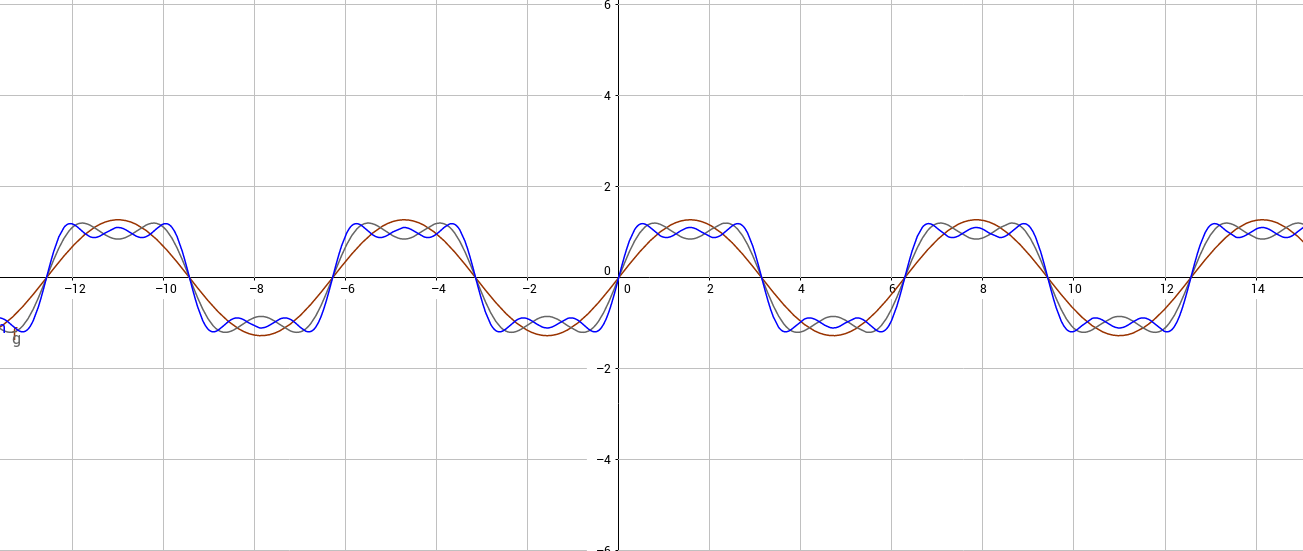
\includegraphics[width=350pt]{Signal_carre_fourier.png}
		\caption{Approximation de la fonction carrée par $S_1$, $S_3$ et $S_5$}
	\end{figure}
	
	\end{myexmpl}
	
	\subsection{Transformée de Fourier}
		La transformée de Fourier permet d'étendre les notions abordées dans le cadre des séries de Fourier dans un cadre plus général, notamment pour des fonctions non périodiques. 
		Dans ce cadre, on ne peut plus se restreindre à la famille des $e_k$ définie précédemment, car la notion de pulsation n'est plus valable dans ce cadre. 
	
	\begin{mydef}
		Soit $f$ une fonction de $L^1(\mathbb{R})$ à valeurs réelles ou complexes. La \textit{Transformée de Fourier} est une fonction complexe définie par :
		$$ \mathcal{F}[f](\xi) = F(\xi)= \int_{-\infty}^{+\infty}f(t)e^{-i\xi t}dt $$ 
	\end{mydef}

	\begin{myrem}
		La condition que la fonction $f$ soit intégrale est suffisante pour que l'intégrale soit bien définie et que la transformée de Fourier existe. 
		De plus, $F(\xi)$ sera une fonction continue et bornée qui tend vers 0 lorsque $|\xi| \longrightarrow \infty$.
		
		En effet, $|f(t)e^{-i \xi t}| \leqslant |f(t)|$ et à $t$ fixé $\xi \mapsto f(t) e^{- i \xi t}$ est continue.
	\end{myrem}
	
	\begin{myproof}
		Soit $f \in L^1(\mathbb{R})$, montrons que $f(\xi) \to 0$ quand $|\xi| \to \infty$. On peut se contenter de le prouver pour un sous ensemble $E$ dense dans $L^1(\mathbb{R})$ (hypothèse $(*)$). En effet soit $\varepsilon > 0$, il existe $h \in E$ tel que $\|f - g\|_1 < \varepsilon / 2$, on a ainsi les calculs suivants :
		
		\begin{align*}
			|\hat{f}(\xi)| & = \left|\int_\mathbb{R} f(t) e^{-i \xi t} dt\right| \\
			& \leqslant \left|\int_\mathbb{R} (f(t) - h(t))e^{- i \xi t} dt\right| + \left|\int_\mathbb{R} h(t) e^{- i \xi t}\right| \quad \text{par l'inégalité triangulaire} \\
			& \leqslant \int_{\mathbb{R}} |f(t) - h(t)| dt + \left|\int_\mathbb{R} h(t) e^{- i \xi t}\right| \\
			&= \varepsilon / 2 + \left|\int_\mathbb{R} h(t) e^{- i \xi t}\right| \\
			&= \varepsilon/2 + \varepsilon/2 \quad \text{pour $\xi$ assez grand par l'hypothèse } (*)
		\end{align*}
		
		L'hypothèse $(*)$ est bien vérifiée pour $E$ étant l'espace des fonctions continûment dérivables et à support compact. Soit $g \in E$, disons définie sur $[a, b]$, on a grâce à une intégration par partie :
		
		$$\int_{a}^{b} f(t) e^{- i \xi t} dt = \frac{i}{\xi} f(t) e^{- i \xi t} \bigg\vert_{t = a}^{t=b} - \frac{i}{\xi} \int_{a}^{b} f'(t) e^{- i \xi t} dt \longrightarrow 0 \quad (|\xi| \to \infty)$$
		
		\cqfd
	\end{myproof}
	
	Nous pourrons nous restreindre aux fonctions de $L^1$ pour cette étude. 
	Comme pour l'étude des séries de Fourier, une notion très importante est de pouvoir reconstruire le signal à partir de sa transformée de Fourier. Pour ce faire, il est possible d'utiliser la transformée de Fourier inverse. 

	\begin{mydef}
		En ajoutant la condition que $f$ soit continue aux conditions précédentes, on peut définir la \textit{transformée de Fourier inverse} par :
		$$ \overline{\mathcal{F}}[F](t) = f(t)=\frac{1}{{2\pi}} \int_{-\infty}^{+\infty}F(\xi)e^{i \xi t}dt $$ 
	\end{mydef}
	
	\begin{myrem}
		Si la condition de la continuité de $f$ n'est pas respectée, la transformée de Fourier de $f$ sera quand même définie, mais l'égalité entre $f$ et $\overline{\mathcal{F}}[\mathcal{F}[f]]$ ne sera vérifiée que presque partout. 
	\end{myrem}
			
	\begin{myexmpl}
		Soit $f \in L^1(\mathbb{R})$ une fonction définie par 	
		$ f(t) = \left\{
		\begin{array}{cc}
		1 & \text{ sur }[-a; a] \\
		0 & \text{sinon} \\
		\end{array}
		\right. $.
		Calculons sa transformée de Fourier: 
		\begin{align*}
			\mathcal{F}[f](\xi)& = \int_{- \infty}^{+\infty} f(t)e^{-i\xi t}dt \\
							   & = \int_{-1}^{1} e^{-i\xi t}dt \\
							   & =  \left[ -\frac{e^{-i\xi t}}{i \xi} \right]_{-a}^{a} \\
							   & =  \frac{-e^{-ia\xi} + e^{ia \xi}} {i \xi} \\
							   & = \frac {2 \sin{a\xi}}{\xi} \qquad \text{d'après la formule d'Euler}
		\end{align*}
		
			\begin{figure}[h]
				\centering
				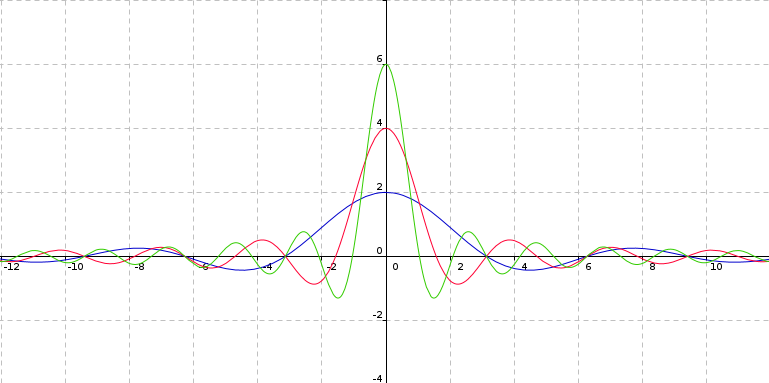
\includegraphics[width=350pt]{TF123.png}
				\caption{Transformée de Fourier de f pour a = 1, 2, 3}
			\end{figure}
	\end{myexmpl}
	
	\subsection{Transformée de Fourier à fenêtre glissante}
	La transformée de Fourier à fenêtre glissante est une solution par rapport au problème de la notion de temporalité apporté par l'étude de signaux continus et non plus périodiques. 

	En reprenant la définition de la transformée de Fourier précédente, on peut l'étendre pour ajouter la notion de fenêtre glissante. 
		
	\begin{mydef}
		Soit $f$ une fonction qui possède une transformée de Fourier. On peut définir la \textit{Transformée de Fourier à fenêtre glissante} par :
		$$ F(\xi, \tau)= \int_{-\infty}^{+\infty}f(t)e^{-i \xi t} \overline{w(t - \tau)}dt$$
		où $w$ est la fonction de fenêtrage, et $\tau$ le paramètre de translation. 
	\end{mydef}
	Il s'agit ensuite de trouver le format de fenêtre adéquat. La fonction la plus simple à imaginer est sans doute la fonction "porte" définie par 
	$w(t) = \left\{
		\begin{array}{cc}
		1 & \text{ sur }[-1; 1] \\
		0 & \text{sinon} \\
		\end{array}
	\right. $.
	Cependant, il en existe de nombreuses autres dont on parlera plus tard. 
	
	\begin{myrem}
		Il existe également une transformée inverse pour la transformée de Fourier à fenêtre glissante. 
	\end{myrem}
	
	\subsection{Transformée de Fourier discrète}
			
	Ces conditions sont nous permettent de définir un cadre pour utiliser la transformée de Fourier. Néanmoins, lors d'applications à l'informatique, nous ne pouvons pas conserver une infinité de valeurs, et il est nécessaire de pouvoir travailler sur des valeurs discrètes, tout en conservant au plus les propriétés pour décomposer et recomposer les fonctions. 		
	Dans le cadre de la transformée de Fourier discrète, au lieu d'utiliser des fonctions, nous allons nous intéresser à des suites qui correspondront à l'échantillonnage de la fonction. Il est important de noter que ces suites seront finies, pour correspondre à l'espace de stockage fini des ordinateurs. 
	

	\begin{mydef}
		On définit la fréquence d'échantillonnage comme le nombre d'échantillons par unité de temps.  
	\end{mydef}
		Pour que l'échantillonnage soit suffisant pour obtenir une reconstitution de qualité suffisante, on peut se référer au théorème de Nyquist-Shannon. 
		
	\begin{mythm}
		Si une fonction $f(t)$ ne contient pas de fréquences plus élevées que $B$ Hz, il est complètement décrit en donnant une suite de ses valeurs a des points régulièrement espacés tout les $\frac{1}{2B}$ secondes.
	\end{mythm}
	
	Dans la mesure où tous les appareils utilisés pour enregistrer des signaux ne peuvent pas capter de valeurs infinies, il sera possible de reconstituer le signal à partir de cette suite de valeurs, avec pour limite la qualité des appareils d'enregistrements et non pas les outils mathématiques. Dans certains cas, l'acuité humaine peut également servir de limite.
	
	\begin{myexmpl}
		 Pour les enregistrements audios, la fréquence d'échantillonnage des fichiers pour le format CD est traditionnellement de 44 100 Hz, ce qui est juste supérieur au double de la fréquence la plus élevée que peut percevoir l'oreille humaine en théorie, c'est à dire 20 000 Hz. 
	\end{myexmpl}
	
	\begin{mydef}
			On considère une suite $(s_n)_{n\in \{0; N -1 \}}$ de N termes. La transformée de Fourier Discrète permet d'obtenir la suite  $(S_n)_{n\in \{0; N -1 \}}$ de N termes définis par :
			$$ S_k = \sum_{k=0}^{N-1}s_n e^{-2i\pi k\frac{n}{N}} $$
	\end{mydef}
		De la même manière que pour la transformée de Fourier, on pourra également définir la transformation inverse.
		
	\begin{mydef}
		Dans les mêmes conditions que ci dessus, on définit la transformée de Fourier discrète inverse par :
			$$ s_n =\frac{1}{N} \sum_{k=0}^{N-1}S_k e^{2i\pi k\frac{n}{N}} $$
	\end{mydef}
	
	Ces transformations sont sans pertes d'informations, ainsi, si les conditions du théorème de Nyquist-Shannon sur la fréquence d'échantillonnage ont été respectées, alors le signal peut être reconstitué sans perte via ces transformations successives. 
	
	L'avantage de l'utilisation de la transformée de Fourier discrète se retrouve également dans la vitesse d'exécution des calculs. En effet, la transformée de Fourier continue à d'un échantillon de N termes a une complexité en $O(N^2)$ alors qu'il existe des algorithmes comme celui de La transformée de Fourier rapide, qui sous certaines conditions sur le nombre de termes de la suite à transformer, par exemple être une puissance de 2, peuvent atteindre une complexité en $O(N\log(N))$. 
	
	Dans le cas classique, pour calculer chacun des $N$ coefficients, il faut effectuer $N$ multiplications, d'où une complexité en $O(N)$.
	Dans le cas de l'algorithme de Cooley-Tukey, si $N$ est une puissance de 2, alors il est possible de réécrire la somme $S_N$ en deux sommes, l'une sur les termes pairs et l'autre sur les termes impairs. Ces deux sommes sont des transformées de Fourier discrètes sur $N/2$ points. Grâce à la périodicité de la transformée de Fourier, on peut déduire que si $S_k = P_k + I_k$, avec $P_k$ et $I_k$ les transformées sur les termes pairs et impairs de longueur $ N/2$, alors $ S_{k+\frac{N}{2}} = P_k + I_k$.  Récursivement, on peut appliquer cette décomposition pour calculer $P_k$ et $I_k$, ce qui nous donne la complexité attendue. 
	
	
\end{document}

	\documentclass[]{article}
\usepackage[utf8]{inputenc}
\usepackage{pdfpages}
\usepackage{amsmath}
\usepackage{amssymb}
\usepackage{graphicx}
\usepackage{geometry}
\usepackage{enumitem}
\usepackage{amsthm}
\usepackage{stmaryrd}
\usepackage{mathtools}
\usepackage{mathrsfs}
\usepackage{bbm}

\geometry{hmargin=2cm}

% Environnement type théorème
\newtheorem{mythm}{Théorème}
\newtheorem{myproposition}{Proposition}
\newtheorem{myproperty}{Propriété}
\newtheorem{mylemma}{Lemme}
\newtheorem{mycoro}{Corollaire}

% Environnement type texte
\theoremstyle{remark}
\newtheorem{mynot}{Notation}
\newtheorem{myrem}{Remarque}
\newtheorem{myexer}{Exercice}
\newtheorem{myproof}{Preuve}
\newtheorem{myexmpl}{Exemple}

% Environnement de définition
\theoremstyle{definition}
\newtheorem{mydef}{Définition}
\newtheorem{myquestion}{Question}

\setlist[itemize]{label=-}

% Carré de fin de preuve
\newcommand{\cqfd}{
	\hfill$\square$
}

% Définition de fonction
\newcommand{\func}[5]{
#1 ~ : ~ \left\{ \begin{array}{lcl}
	#2 & \longrightarrow & #3 \\
	#4 & \longmapsto & #5
\end{array}
\right.
}

\newcommand{\fun}[3]{
#1 ~ : ~ #2 \longrightarrow #3
}

\newcommand{\funcinline}[5]{
	#1 \, : \, #2 \longrightarrow #3, ~ #4 \longmapsto #5
}

\newcommand{\funcshort}[3]{
	#1 \, : \, #2 \longrightarrow #3
}

\newcommand{\anonfunc}[4]{
	\left\{ \begin{array}{lcl}
		#1 & \longrightarrow & #2 \\
		#3 & \longmapsto & #4
	\end{array}
	\right.
}

\allowdisplaybreaks[4]

\newcommand{\vect}{\text{Vect}}

\newcommand{\card}{\text{Card }}

\newcommand{\DS}{\displaystyle}

\begin{document}
	\part{Analyse du signal}
	
	On munit à présent $L^2(\mathbb{R})$ du produit scalaire $\langle \cdot, \cdot \rangle$ défini par $$\langle f, g\rangle = \int_\mathbb{R} f(t) \overline{g(t)} dt$$
	et de la topologie induite par la norme correspondante.
	
	\section{Analyse multi-résolution}
	
	\subsection{Introduction}
	
	Nous allons enrichir la théorie des espaces de Hilbert d'une notion de "finesse"  particulièrement adaptée à l'objet central de ce rapport. En effet, dans le cadre de l'approximation d'un signal, que nous modélisons par une fonction $\mathbb{R}^n \rightarrow \mathbb{R}^m$, cette notion prend tout son sens comme le montre l'image ci-dessous.
	
	\begin{figure}[h]
		\centering
		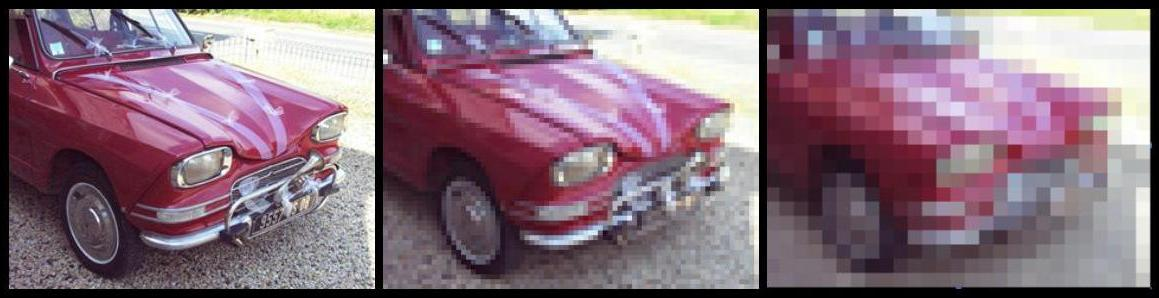
\includegraphics[width=350pt]{Resolution_wikipedia.jpg}
		\caption{Une image de voiture pour trois résolutions différentes}
	\end{figure}
	
	Les images peuvent être modélisées comme des fonctions de $\mathbb{R}^2$, pour les coordonnées spatiales, dans $\mathbb{R}$ (resp. $\mathbb{R}^3$) dans le cas d'une image en noir et blanc (resp. en couleur RVB). Dans le cas d'un signal sonore, sachant qu'un son est une onde, il peut être représenté par une fonction de $\mathbb{R}$, pour le temps, dans $\mathbb{R}$, pour l'amplitude de d'oscillation.
	
	Avant de définir l'analyse multi-résolution, explorons plus profondément cette notion de "finesse".
	
	\subsubsection*{Quelle finesse !}
	
	Nous allons prendre pour exemple les signaux unidimensionnels (tels les sons). Soit $\funcshort{f}{[0, 1[}{\mathbb{R}}$ une fonction continue, nous allons l'approximer par des fonctions constantes par morceaux (dites étagées), dont les morceaux sont de plus en plus petits.
	
	\begin{figure}[h]
		\label{sine-stairs}
		\centering
		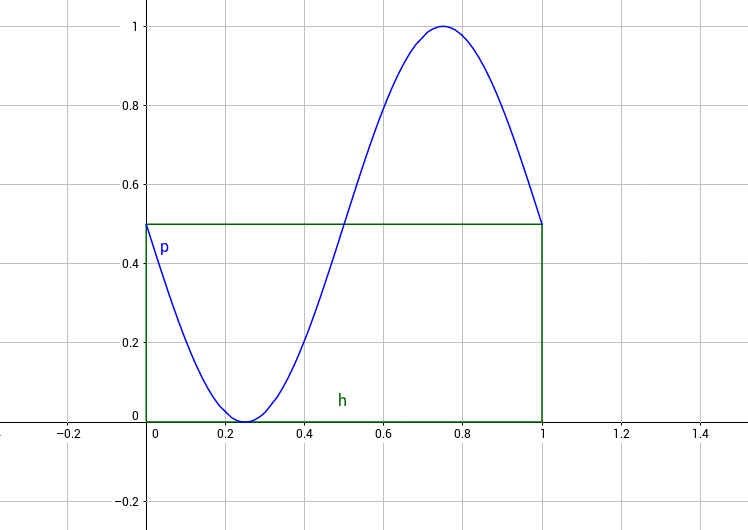
\includegraphics[width=150pt]{sin_1.png}
		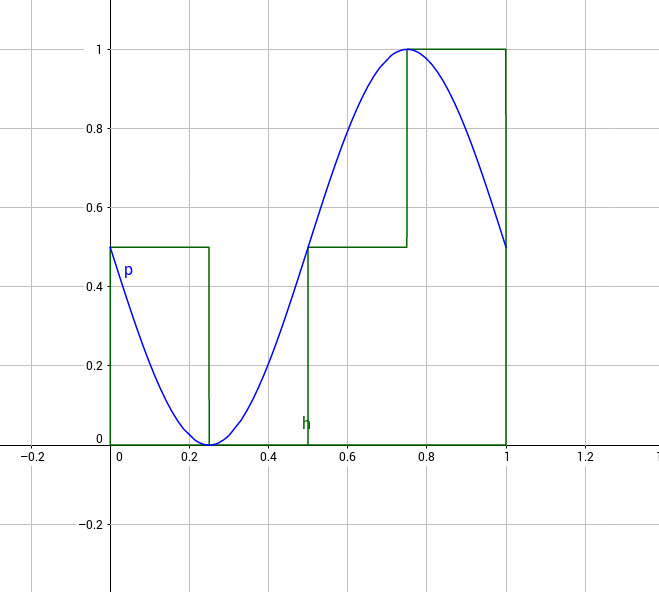
\includegraphics[width=150pt]{sin_2.png}
		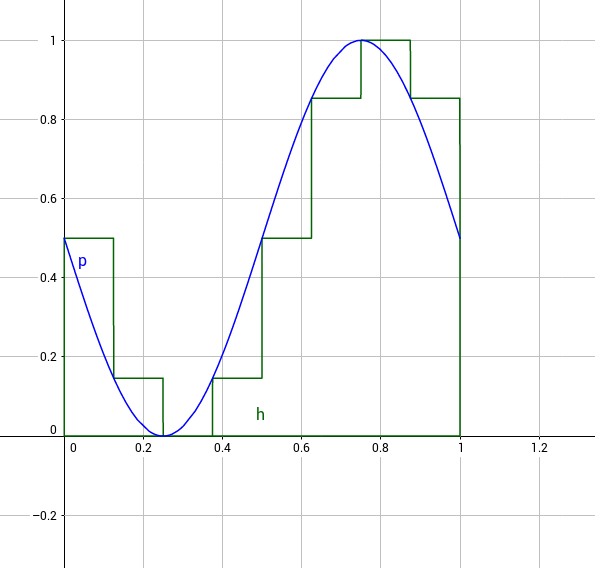
\includegraphics[width=150pt]{sin_4.png}
		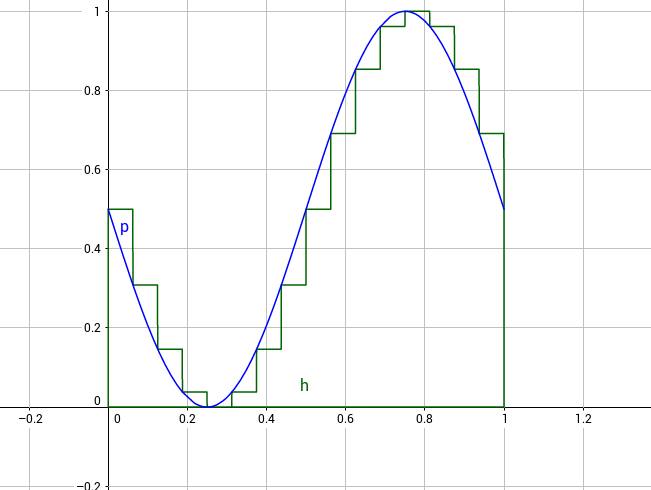
\includegraphics[width=150pt]{sin_8.png}
		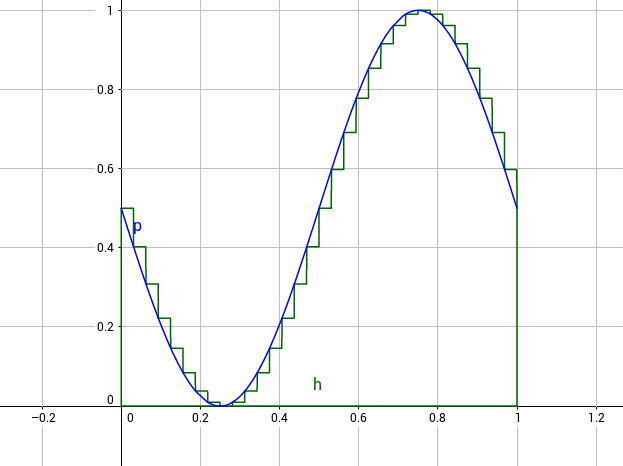
\includegraphics[width=150pt]{sin_16.png}
		\caption{$f$ approximée par des fonctions dont les morceaux sont de tailles 1, 1/2, 1/4, 1/8 et 1/16}
	\end{figure}
	
	\newpage
	
	Sur la figure on approxime $f$ par des fonctions $f_n$ étagées dont les morceaux sont de tailles $2^{-n}$, on peut voir chaque $f_n$ comme une combinaison linéaire de fonctions caractéristiques de la forme suivante $$f_n = \sum_{k = 0}^{2^n} a_{n, k} \mathbbm{1}_{[k 2^{-n}, (k+1)2^{-n}[}$$
	
	La première remarque que l'ont peut faire est que chaque $\mathbbm{1}_{[k 2^{-n}, (k+1)2^{-n}[}$ est le translaté de $\mathbbm{1}_{[0, 2^{-n}[}$, que l'on notera $I_n$. On réécrit alors $$f_n(x) = \sum_{k = 0}^{2^n} a_{n, k} I_n\left(x - k 2^{-n}\right)$$
	
	La seconde est que $I_n$ est une contraction de $I_1$ que l'on notera $I$. On en tire notre dernière réécriture :
	
	$$f_n(x) = \sum_{k = 0}^{2^n} a_{n, k} I \left(\frac{x - k 2^{-n}}{2^{-n}}\right) = \sum_{k = 0}^{2^n} a_{n, k} I \left(2^n x - k\right)$$
	
	Ainsi si on fixe $I = \mathbbm{1}_{[0, 1[}$ comme fonction de référence dans notre décomposition, la suite de fonctions $(f_n)_n$ est entièrement déterminée par les coefficients $(a_{n, k})_{n, k}$
	
	\subsection{L'analyse multi-résolution}
	
	Dans l'exemple introductif, pour tout $n$ on a pu voir que $f_n$ était une combinaison linéaire du translaté d'une fonction $I_n$, $f_n$ appartenait alors à l'espace vectoriel engendré par les translations de $I_n$. De plus, chaque $I_n$ était la contraction de la fonction $I$ donnée par $I_n(t) = I\left(t 2^n\right)$. Il s'agissait d'un exemple d'analyse multi-résolution dont voici la définition :
	
	\begin{mydef}
		Une \textit{analyse multi-résolution} de l'espace $L^2(\mathbb{R})$ des fonctions de carré Lebesgue-intégrables est une suite $V = \{V_n\}_{n \in \mathbb{Z}} \subset L^2(\mathbb{R})$ de sous-espaces fermés de $L^2(\mathbb{R})$ satisfaisant aux conditions suivantes :

		\begin{equation}
			\label{growth}
			\forall n \in \mathbb{Z}, ~ V_{n} \subset V_{n+1} \text{ (croissance)}
		\end{equation}
		\begin{equation}
			\label{self-similarity}
			\forall n \in \mathbb{Z}, \forall f \in L^2(\mathbb{R}), ~ f \in V_n \Longleftrightarrow f (2 \, \cdot ) \in V_{n+1} \text{(auto-similarité)}
		\end{equation}
		\begin{equation}
			\label{rb-mra}
			\text{Il existe $\varphi$ telle que $\{\varphi(\, \cdot + k)\}_{k \in \mathbb{Z}}$ forme une base orthonormée de $V_0$}
		\end{equation}
		\begin{equation}
			\label{density}
			\overline{\bigcup V} = L^2(\mathbb{R}) \text{(densité)}
		\end{equation}
		\begin{equation}
			\label{inter}
			\bigcap V = \{0\}
		\end{equation}
		
		$\varphi$ est appelée \textit{fonction d'échelle}.
	\end{mydef}
	
	On peut généraliser par récurrence la propriété \ref{self-similarity} de la façon suivante :
	\begin{equation}
		\forall n \in \mathbb{Z}, \forall f \in L^2(\mathbb{R}), ~ f \in V_0 \Longleftrightarrow t \mapsto f \left(2^n t\right) \in V_{n}
	\end{equation}

	Ce qui met en évidence que plus $n$ est grand, plus l'espace $V_n$ contient des fonctions fines (la fonction est contractée horizontalement). D'après les propriétés \ref{self-similarity} et \ref{rb-mra}, on peut déduire que toute fonction de $V_n$ est une combinaison linéaire de contraction (d'un facteur au plus $2^n$) et translation de $\varphi$.

	\begin{mydef}
		Une analyse multi-résolution est dite \textit{localisée} si $\varphi$ vérifie la condition suivante
		\begin{equation}
			\label{localized}
			\forall m \in \mathbb{N}, \int_\mathbb{R} (1+|t|)^m |\varphi(t)|^2 dt < + \infty
		\end{equation}
	\end{mydef}
	
	Cette propriété porte bien son nom, si $\varphi$ la vérifie alors $|\varphi|^2$ décroît bien plus vite que tout polynôme en $\pm \infty$, suffisamment pour être intégrable. C'est le cas par exemple des gaussiennes et des fonctions à support compact. Une telle fonction $\varphi$ a une masse concentrée près de 0, ce qui limitera les "interférences" de ses translations dans leurs combinaisons linéaires.
	
	\begin{figure}[h]
		\centering
		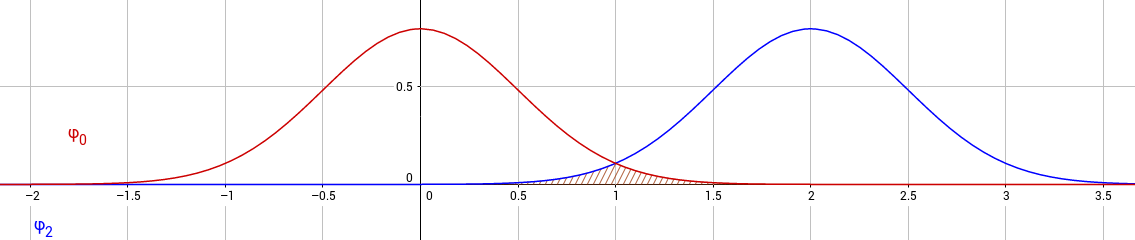
\includegraphics[width=450pt]{Localized.png}
		\caption{Les gaussiennes sont localisées}
	\end{figure}
	
%	\begin{myexmpl}
%		On reprend l'exemple précédent, avec $\varphi = \mathbbm{1}_{[0, 1[}$. On a alors pour tout $n, k \in \mathbb{Z}$ $$\varphi_{n, k} = 2^{n/2} \mathbbm{1}_{[k 2^{-n}, (k+1) 2^{-n}[}$$
%		
%		Pour tout entier $n$, la famille $\left(\varphi_{n, k}\right)_{k \in \mathbb{Z}}$ est effectivement une famille orthonormée : 
%		\begin{align*}
%			\langle \varphi_{n, k}, \varphi_{n, k'} \rangle &= \int_{\mathbb{R}} \varphi_{n, k} \varphi_{n', k'} d \lambda \\
%			&= \int_{\mathbb{R}} 2^{-n}  \mathbbm{1}_{[k 2^{-n}, (k+1) 2^{-n}[} \mathbbm{1}_{[k' 2^{-n}, (k'+1) 2^{-n}[} d \lambda \\
%			&= 2^{n}  \int_{\mathbb{R}} \mathbbm{1}_{[k 2^{-n}, (k+1) 2^{-n}[ \cap [k' 2^{-n}, (k'+1) 2^{-n}[} d\lambda \\
%			&= 2^{n} \lambda\left([k 2^{-n}, (k+1) 2^{-n}[ \cap [k' 2^{-n}, (k'+1) 2^{n}[\right)
%		\end{align*}
%		
%		On voit bien que les ensembles $[k 2^{-n}, (k+1) 2^{-n}[$ sont disjoints, donc la mesure de l'intersection considérée est soit nulle (si $k \neq k'$), soit égale à $\lambda([k 2^{-n}, (k+1) 2^{-n}[) = 2^{-n}$ (si $k = k'$).
%		
%		On retrouve bien $$\langle \varphi_{n, k}, \varphi_{n, k'} \rangle = \delta_{k, k'}$$
%		
%		On peut de plus approximer toute fonction de $L^2(\mathbb{R})$ aussi finement que souhaité par une fonction de $\DS \bigcup_{n \in \mathbb{Z}} V_n$.
%		
%		* Mq $V_n$ fermé
%		
%		* Mq toute fonction peut être approximé avec une finesse arbitraire par un élément de $\bigcup V$
%	\end{myexmpl}
		
	\newpage
		
	\subsection{Espace des détails}
	
	Pour tout $n$, on dénote par $\funcshort{P_n}{L^2(\mathbb{R})}{V_n}$ la projection orthogonale sur $V_n$ (on choisit les projections orthogonales car elles minimisent l'erreur commise en passant d'un espace à l'autre). Ainsi, pour tout $f \in L^2(\mathbb{R})$, $P_n (f)$ est l'approximation de $f$ avec une précision $2^{-n}$. Sur la figure $\ref{sine-stairs}$, on projette $f$ sur les espaces $V_0$ à $V_4$.
	
	Penchons nous sur ce qui se passe lorsqu'on passe d'une échelle plus fine à une échelle plus grossière.
	
	Soient $f \in L^2(\mathbb{R})$ et $f_n$ son approximation dans $V_n$ (c'est-à-dire $f_n = P_n(f)$). Le passage de $V_n$ à $V_{n-1}$ constitue une perte d'informations car on passe d'un espace plus fin à un espace plus grossier.
	
	\begin{align*}
		f_{n-1} &= P_{n-1} (f_n) \\
		&= P_{n-1}( (f_n - f_{n-1}) + f_{n-1}) \\
		&= \underbrace{P_{n-1} (f_n - f_{n-1})}_{0} + f_{n-1} \\
	\end{align*}
	
	La perte de précision, formalisée par $f_n - f_{n-1}$, est donc un élément du noyau de $P_{n-1}$, à savoir $V_{n-1}^\bot$. Mais $f_n - f_{n-1}$ étant dans $V_{n}$, l'ensemble regroupant les détails perdus en passant de $V_n$ à $V_{n-1}$ est $V_{n-1}^\bot \cap V_n$, c'est-à-dire le complémentaire orthogonal de $V_{n-1}$ dans $V_n$.
	
	\begin{mydef}
		Pour tout $n$ on définit \textit{l'espace de détails} $W_{n}$ comme le complémentaire orthogonal de $V_{n}$ dans $V_{n+1}$ $$V_{n+1} = W_n \stackrel{\perp}{\oplus} V_n$$
	\end{mydef}
	
	\paragraph*{}
	Les $(W_n)_n$ ne forment plus une famille monotone, mais leur somme recouvre tous les $V_n$. En d'autre termes, on peut à présent approximer toute fonction de $L^2(\mathbb{R})$ par une combinaison linéaire d'éléments de $\DS \bigoplus_{n \in \mathbb{Z}} W_n$.
	
	\begin{myproof}
		Soit $n_0 \in \mathbb{Z}$, on a par définition des $(W_{n})_n$
		
		\begin{align*}
			V_{n_0+1} &= V_{n_0} \oplus W_{n_0} \\
			&= V_{n_0 - 1} \oplus \left(W_{n_0 - 1} \oplus W_{n_0} \right) \\
			& \cdots \\
			&= V_{n_0 - N} \oplus \left(\bigoplus_{n = n_0 - N}^{n_0} W_n \right) \\
			& \cdots \\
			&= \bigcap V \oplus \left(\bigoplus_{n = - \infty}^{n_0} W_n \right) \\
			&= \{0\} \oplus \left(\bigoplus_{n = - \infty}^{n_0} W_n \right) \\
			&= \bigoplus_{n = - \infty}^{n_0} W_n
		\end{align*}
		
		On en déduit ainsi $\DS \bigcup V = \bigoplus_{n \in \mathbb{Z}} W_n$ en faisant tendre $n_0$ vers $\infty$ (ou plutôt en faisant l'union à gauche et à droite pour tout $n_0 \in \mathbb{Z}$).
		
		\cqfd
	\end{myproof}
	
	Comme on l'a dit, les $(W_n)_n$ ne forment pas une suite d'espaces emboîtés (ils sont même orthogonaux deux à deux), cependant ils vérifient encore les conditions d'auto-similarité et de stabilité par translation.

	\section{Ondelettes}

	\begin{mydef}
		Il existe une fonction normée $\psi$ - appelée \textit{ondelette} - engendrant $W_0$ par translation et de moyenne nulle (d'intégrale nulle).
		
		On admettra son existence \footnote{Voir \textit{Wavelets and Multiscale Signal Processing} d'Albert Cohen pour une démonstration de l'existence.}, mais elle peut être construite explicitement à partir de $\varphi$.
	\end{mydef}
		
	On définit encore une fois la famille $\Psi = \{\psi_{n, k}\}_{n, k \in \mathbb{Z}}$ par $\psi_{n, k}(t) = 2^{-n/2} \psi(2^{n} t - k)$, et cette fois ci ... cette famille est une base orthonormée de $\DS \bigoplus_{n \in \mathbb{Z}} W_n$ ! Et donc une base hilbertienne de $L^2(\mathbb{R})$ !
	
	Le fait que la famille soit normée est évident, le fait qu'elle soit orthogonale découle de l'orthogonalité des $W_n$.
	
	\begin{myexmpl}
		On prend comme exemple l'ondelette de Haar qui est donnée par $$\psi(t) = \left\{
		\begin{array}{cl}
			0 & x < 0 \\
			1 & 0 \leqslant x < \frac{1}{2} \\
			-1 & \frac{1}{2} \leqslant x < 1 \\
			0 & 0 \leqslant x
		\end{array}
		\right.$$
	\end{myexmpl}
	
	\begin{figure}[h]
		\label{Haar}
		\centering
		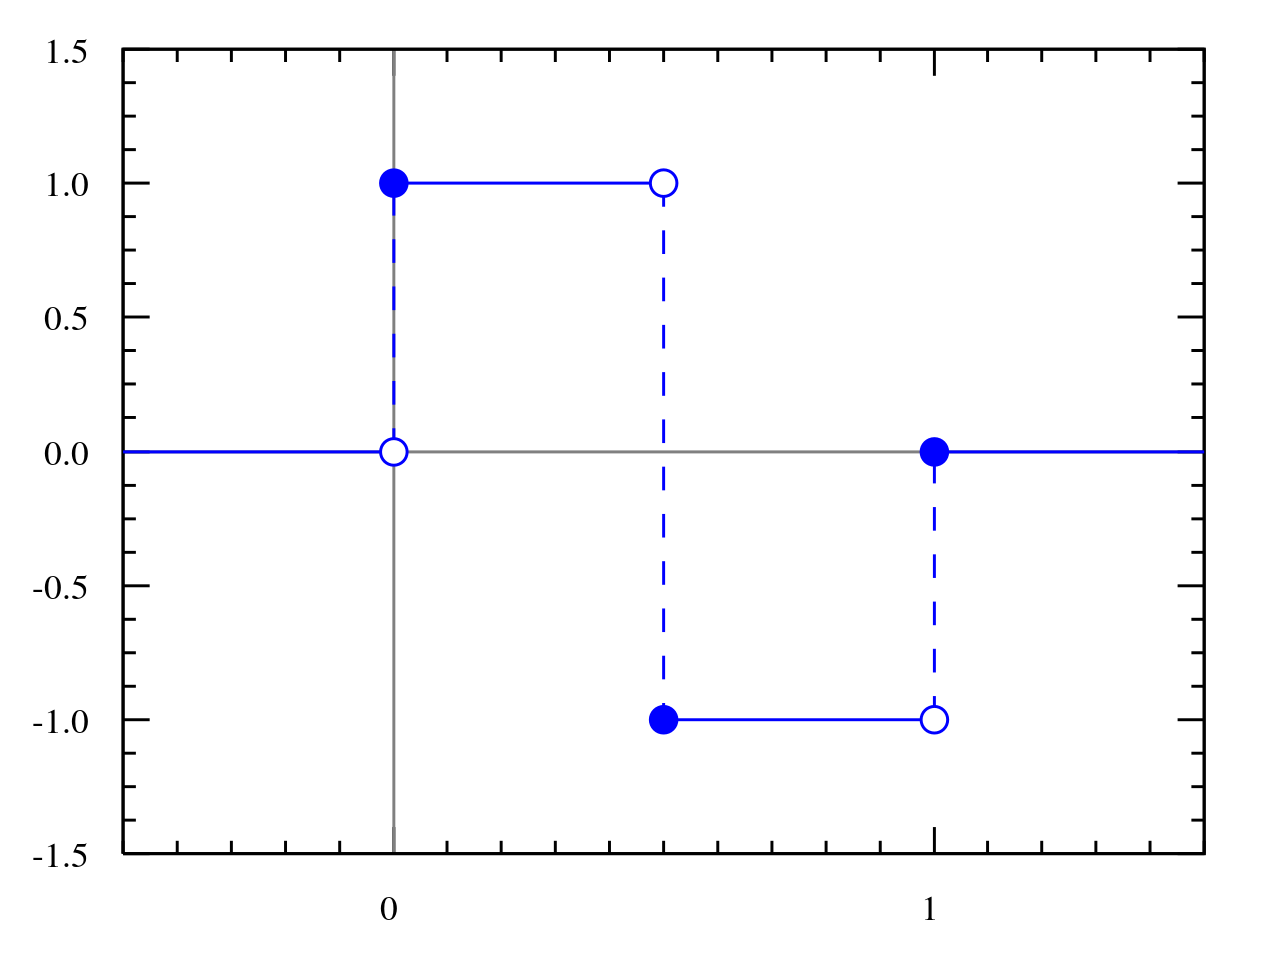
\includegraphics[width=150pt]{Haar.png}
		\caption{L'ondelette de Haar}
	\end{figure}
	
	$\psi$ est effectivement de moyenne nulle et $\Psi$ est orthonormée :
	
	\begin{align*}
		\langle \psi_{n, k}, \psi_{m, l}\rangle &= \int_{-\infty}^{\infty} \psi_{n, k}(t), \psi_{m, l}(t) dt \\
		&= 2^{\frac{m+n}{2}} \int_{-\infty}^{\infty} \underbrace{\psi(2^nt - k) \psi(2^mt - l)}_{h(t)} dt
	\end{align*}
	
	Si le graphe de la fonction $h$ admet un centre de symétrie sur $\mathbb{R}$ alors elle sera d'intégrale nulle (généralisation du fait que l'intégrale d'une fonction impaire est nulle). Cette remarque nous fournit un argument géométrique pour justifier que $\langle \psi_{n, k}, \psi_{m, l}\rangle$ vaut 1 si $n = m$ et $k = l$, et 0 sinon.
	
	Supposons $n \neq m$, alors les fonctions peuvent se positionner l'une par rapport à l'autre de quatre façons différentes, leur produit aura bien un centre de symétrie comme sur le figure.
		
	\begin{figure}[h]
		\centering
		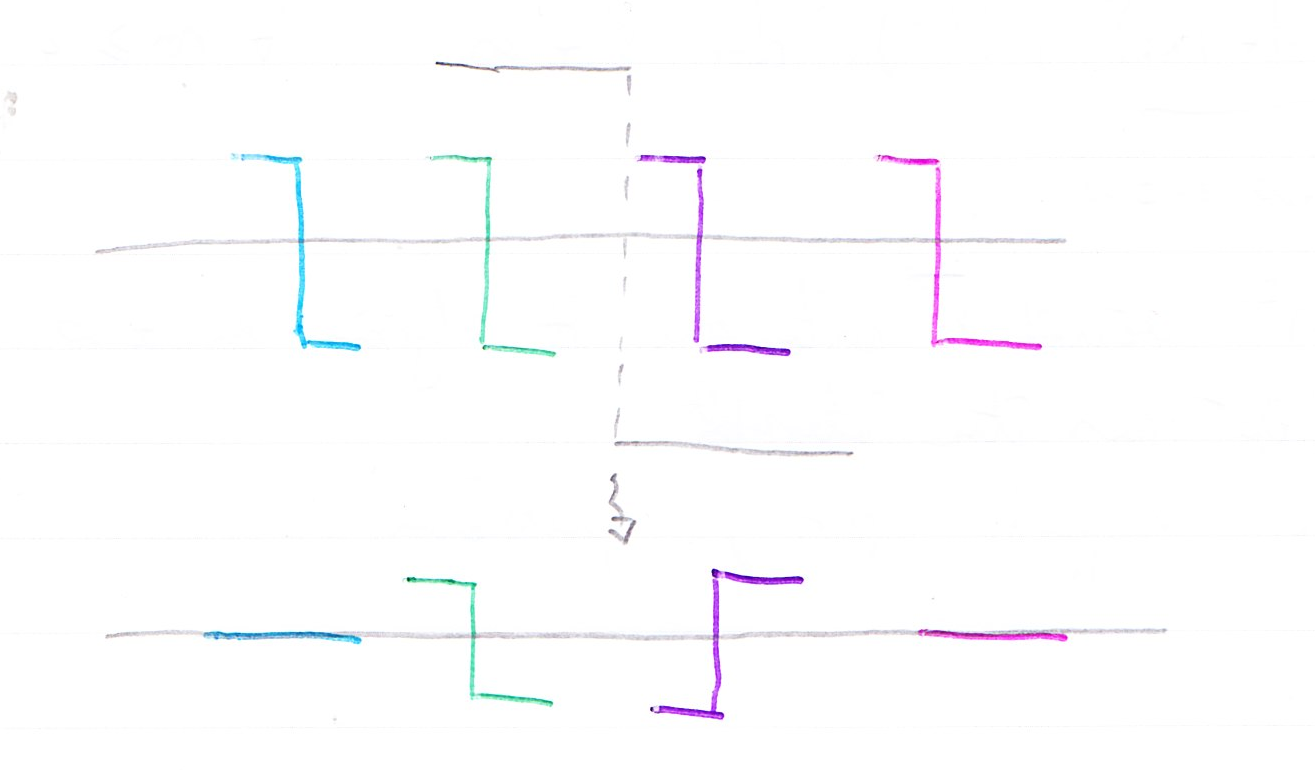
\includegraphics[width=350pt]{Haar_exemple.png}
		\caption{Le produit de deux ondelettes de Haar différentes  (la grise par une en couleur) possèdent un centre de symétrie dans $\mathbb{R}$.}
	\end{figure}
	
	\begin{myexmpl}
		Voici un autre exemple d'ondelette appelée "Chapeau mexicain" (ou ondelette de Ricker) est définie comme la dérivée seconde d'une gaussienne. Elle est donnée par 
		
		$$\psi(t) = \lambda e^{-t^2/2} (1 - t^2)$$
		
		avec $\lambda$ tel que $\|\psi\|_2 = 1$, c'est-à-dire que
		
		\begin{align*}
			1 = \|\psi\|_2^2 &= \lambda^2 \int_{- \infty}^{\infty} e^{-t^2} (1-t^2)^2 \\
			&= \lambda^2 \left(\int_{-\infty}^{\infty} e^{-t^2} dt - 2 \int_{-\infty}^{\infty} t^2 e^{-t^2} dt + \int_{-\infty}^{\infty} t^4 e^{-t^2} dt\right) \\
			&= \lambda^2 \left(\sqrt{2 \pi} - \sqrt{2 \pi} + \frac{3}{2} \sqrt{2 \pi}\right) \\
			&= \lambda^2 \frac{3}{2} \sqrt{2 \pi}
		\end{align*}
		
		donc $\DS \lambda = \frac{2^{3/4}}{\sqrt{3} \pi^{1/4}}$.
		
		\begin{figure}[h]
			\centering
			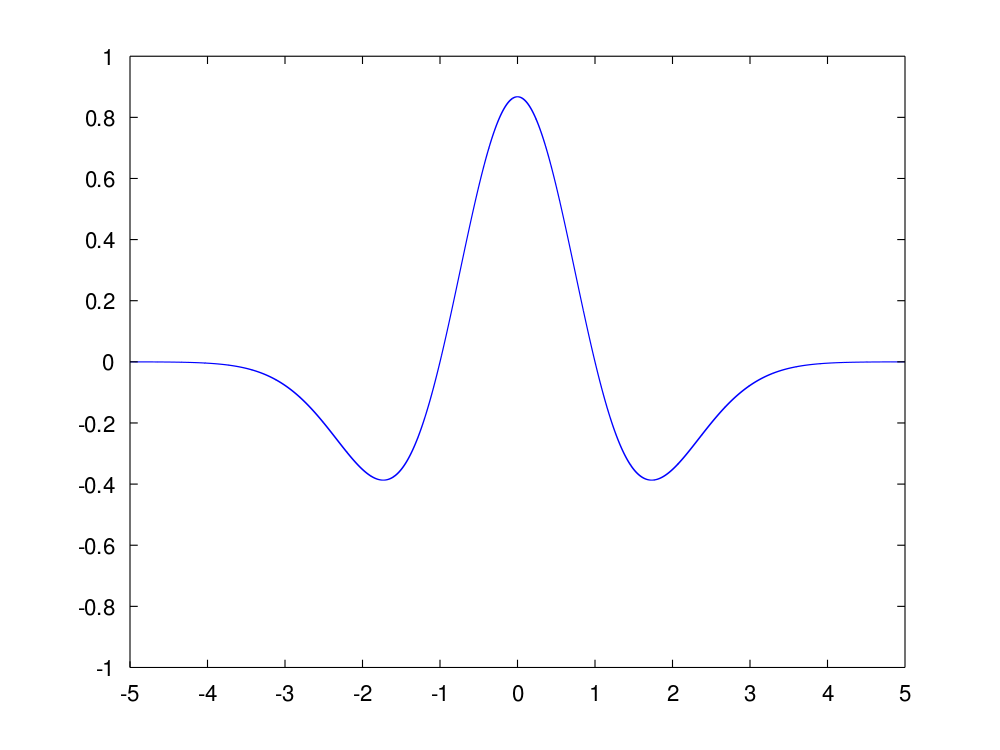
\includegraphics[width=350pt]{Mexican_Hat.png}
			\caption{Le chapeau mexicain}
		\end{figure}
	
		Elle est effectivement de moyenne nulle : si $g$ est une gaussienne telle que $g^{(2)}= \psi$ alors $$\int_{-\infty}^{\infty} \psi(t) dt = g'(t) \bigg\vert_{-\infty}^{\infty} = 0$$

		car $g'(t)$ est de la forme $t e^{-t^2}$.
	\end{myexmpl}
	
	\begin{mydef}
		On dit d'une ondelette qu'elle \textit{a $n$ moments nuls} si pour tout $k = 0, 1 \cdots n$ elle vérifie $$\int_{-\infty}^{\infty} t^k f(t) dt = 0$$
		
		Autrement dit, elle est orthogonale à tout polynôme de degré au plus $n$ (en gardant bien en tête que les polynômes ne sont pas intégrables).
	\end{mydef}
		
	Une telle ondelette permettra d'obtenir une majoration des coefficients de la transformation en ondelette d'une fonction de classe $\mathcal{C}^{n+1}$ à support borné grâce à la formule de Taylor-Lagrange.
	
	Soit $f$ une fonction $n+1$ fois continûment dérivables à support dans un intervalle $I = [-M/2, M/2]$, pour tout point $x_0 \in I$ il existe un polynôme $P$ de degré $n$ tel que pour tout $x \in I$ 
	
	$$f(x) = P(x - x_0) + f^{(n+1)}(c_{x_0, x}) \frac{(x-x_0)^{n+1}}{(n+1)!} \quad \text{avec } |c - x| < |x - x_0|$$
	
	Ce qui nous fournit la majoration
	
	\begin{align*}
		|\langle f, \psi \rangle| &= \left|\int_{-\infty}^{\infty} f(x) \psi(x) dx \right| \\
		&= \left| \int_{-\infty}^{\infty}P(x - x_0) \psi(x) dx + \int_{-\infty}^{\infty} f^{(n+1)}(c_{x_0, x}) \frac{(x-x_0)^{n+1}}{(n+1)!} \psi(x) dx  \right| \\
		&= \left| \int_{-\infty}^{\infty} f^{(n+1)}(c_{x_0, x}) \frac{(x-x_0)^{n+1}}{(n+1)!} \psi(x) dx  \right| \\
		&= \left| \int_{I} f^{(n+1)}(c_{x_0, x}) \frac{(x-x_0)^{n+1}}{(n+1)!} \psi(x) dx  \right| \quad \text{car $f^{(n+1)}$ est à support dans $I$} \\
		& \leqslant \left| \int_{I} \frac{(x-x_0)^{n+1}}{(n+1)!} \psi(x) dx \right| \|f\|_{\infty} \\
		& \leqslant \frac{M^{n+1}}{(n+1)!} \left| \int_{I} \psi(x) dx \right| \|f\|_{\infty} \\
		& \leqslant \frac{M^{n+1}}{(n+1)!} \|f\|_{\infty}
	\end{align*}
\end{document}
	
\newpage

\part{Algorithmes d'encodage et de décodage}

\section{Cadre théorique}

D'un point de vue pratique, les fonctions sont représentées comme des fonctions en escalier, qui de plus sont à support bornés (disons sur $[0, 1[$). C'est-à-dire que l'on manipule des fonctions $f \in L^2(\mathbb{R})$ de la forme $$f = \sum_{j = 0}^{2^{N_0} - 1} a_j \mathbbm{1}_{[2^{-N_0}j, 2^{-N_0}(j+1)[}$$

%On veut trouver les coefficients de $f$ dans l'espace vectoriel $V_{N_0} = V_0 \stackrel{\perp}{\oplus} W_0 \stackrel{\perp}{\oplus} \cdots \stackrel{\perp}{\oplus} W_{N_0}$ .

On rappelle qu'on peut décomposer tout fonction $f \in L^2(\mathbb{R})$ ainsi : $$f = \sum_{k \in \mathbb{Z}} \langle \varphi_{0,k}, f \rangle \varphi_{0,k} + \sum_{\substack{k \in \mathbb{Z} \\ n \in \mathbb{N}}} \langle \psi_{n, k}, f \rangle \psi_{n, k}$$

Le calcul des coefficients s'en retrouve ainsi simplifié :

\begin{align*}
	\langle f, \psi_{n, k} \rangle &= \int_0^1 f(t) \overline{\psi_{n, k}(t)} dt \\
	&= \sum_{j=0}^{N-1} \int_{\frac j N}^{\frac{j+1}N} a_j \overline{\psi_{n, k}(t)} dt \\
	&= \sum_{j=0}^{N-1} \int_{\frac j N}^{\frac{j+1}N} a_j \overline{\frac{1}{\sqrt{2^n}} \psi(2^n t - \frac{k}{N})} dt \\
	&= \frac{1}{\sqrt{2^{3n}}} \sum_{j=0}^{N-1} a_j \int_{2^n \frac{j}N - k}^{2^n\frac{j+1}N - \frac{k}{N}} \overline{\psi(u)} du \quad \text{où $2^nt - \frac{k}{N} = u$} \\
	&= \frac{1}{\sqrt{2^{3n}}} \sum_{j=0}^{N-1} a_j \left(\Psi\left(2^n\frac{j+1}N - \frac{k}{N}\right) - \Psi\left(2^n\frac{j}N - \frac{k}{N}\right)\right) \\
	\langle f, \varphi_{0, k} \rangle &= \int_0^1 f(t) \overline{\varphi_{0, k}(t)} dt \\
	&= \sum_{j=0}^{N-1} \int_{\frac j N}^{\frac{j+1}N} a_j \overline{\varphi_{0, k}(t)} dt \\
	&= \sum_{j=0}^{N-1} \int_{\frac j N}^{\frac{j+1}N} a_j \overline{\varphi(t - k)} dt \\
	&= \sum_{j=0}^{N-1} a_j \int_{\frac{j}N - \frac{k}{N}}^{\frac{j+1}N - \frac{k}{N}} \overline{\varphi(u)} du \quad \text{où $t - \frac{k}{N} = u$} \\
	&= \sum_{j=0}^{N-1} a_j \left(\Phi\left(\frac{j+1}N - \frac{k}{N}\right) - \Phi\left(\frac{j}N - \frac{k}{N}\right)\right)
\end{align*}

où $\Psi$ est une primitive de $\overline{\psi}$, $\Phi$ est une primitive de $\overline{\phi}$ et $N = 2^{N_0}$.

Étant face à des fonctions en escalier avec un pas fixe, on peut les représenter comme des vecteurs de $\mathbb{R}^N$, où la $(j+1)$-ième coordonnée est la valeur prise sur le $(j+1)$-ième intervalle. On note $\tilde{f} = (a_j, a_1 \cdots a_N)$ et $\DS \widetilde{\psi}_{n, k} = \left(\frac{1}{\sqrt{2^{3n}}} (\Psi(2^n j - k) - \Psi(2^n (j+1) - k))\right)_{j = 0, 1 \cdots N - 1}$, on a alors 

$$\langle f, \psi_{n, k} \rangle =\widetilde{\psi}_{n, k} \times \transp{\widetilde{f}}$$

De plus, en définissant $S_n = (\langle f, \psi_{n, k}\rangle)_{k = 0, 1 \cdots s(n)}$, avec $s(n)$ le plus grand $k$ que l'on souhaitera calculer, et

$$P_n = 
\left(
	\begin{array}{c}
		\widetilde{\psi}_{n, 0} \\
		\widetilde{\psi}_{n, 1} \\
		\vdots \\
		\widetilde{\psi}_{n, s(n)} 
	\end{array}
\right)$$

on a enfin $$S_n = P_n\times\transp{\tilde{f} }$$

Chaque $P_n$ est alors le projecteur de $f$ sur l'espace de détails $W_n$, les coefficients sont alors stockés dans le vecteur $S_n$.

\begin{myrem}
	La matrice $\widetilde{f}$ est de taille $1 \times N$, $P_n$ de taille $s(n) \times N$ et $S_n$ de taille $1 \times s(n)$.
\end{myrem}

L'algorithme de compression consiste alors en le remplissage des matrices de projection pour chaque niveau de détail et en la multiplication pour obtenir chaque $S_n$. Nous proposons l'algorithme naïf suivant :

\begin{algorithm}
	\begin{algorithmic}[1]
		\Procedure{Encoder}{$\Psi$, $\widetilde{f}$, $N_0$, $s$}
			\State $S_m := \Phi(1)-\Phi(0)$
			\State $P_0 := $ Construire($\Psi$, 0, $s(0)$)
			\For{$n = 0, 1 \cdots N_0$}
				\State $P_n :=$ Construire($\Psi$, $n$, s(n))
				\State $S_n := P_n\times \transp{\widetilde{f}}$
		
			\EndFor
			\State \Return $S_m,(S_0, S_{-1}, S_{1} \cdots S_{N_0}, S_{-N_0})$
		\EndProcedure

		\Statex

		\Procedure{Décoder}{$\psi$, $S_m$, $A=(\alpha_{n, k})_{n, k}$, $N_0$, $s(n)$}
		\For{$x = 0, 2^{-N_0}, 2\times 2^{-N_0} \cdots, 1$}
		\State $f(x) := S_m$
		\For{$n = 0, 1 \cdots, N_0$}
		\For{$k = 0, 1 \cdots, s(n)$}
		\State $f(x) := f(x) + \alpha_{n, k} \times \psi(2^{-n} x - k)$
		\EndFor
		\EndFor
		\EndFor
		\State \Return $f$
		\EndProcedure
	\end{algorithmic}
\end{algorithm}

\subsection{Validation de l'algorithme}

Vérifier que cet algorithme est correct consiste à vérifier que les approximations que l'on a du faire pour passer de valeurs infinies à des valeurs finies pour $n$ et $k$ ne sont pas préjudiciables à la validité des résultats produits. Il s'agit donc de vérifier que les valeurs de $n$ et $k$ enlevées sont négligeables. En effet,  le reste de l'algorithme ne doit pas donner lieu a des erreurs : la formule utilisée est celle qui a été définie plus tôt, et il est certain de terminer. 

% sensibilité
\subsubsection{Coordonnées $n\geqslant N_0$}

La valeur de $\langle f,\psi_{n,k}\rangle$ représente à peu près la «variation» de $f$ dans l'intervalle $[2^{-n}k,2^{-n}(k+1)]$.

Étant donné que $f$ est échantillonnée avec une fréquence de $2^{-N_0}$, $f$ est constante sur les intervalles $[2^{-n}k,2^{-n}(k+1)]$ pour $n\geqslant N_0$.

Concrètement, pour un $n$ aussi grand, on a $\langle f,\psi_{n,k}\rangle = \int_0^1 f(t) \overline{\psi_{n, k}(t)}dt \approx \int_{2^{-n}k}^{2^{-n}(k+1)} f(t) \overline{\psi_{n, k}(t)}dt$ car on suppose que $\psi_{n,k}$ est négligeable en dehors de $[2^{-n}k,2^{-n}(k+1)]$.

La valeur des coordonnées à ces indices est donc négligeable, car sur l'intervalle $[2^{-n}k,2^{-n}(k+1)]$, la fonction $f$ est constante et $\psi_{n,k}$ est de moyenne nulle.

Dans la pratique, cela correspond a des intervalles qui sont plus petits que la fréquence d'échantillonnage: la fonction est donc constante sur l'intervalle, et comme l'ondelette est de moyenne nulle, les valeurs qui lui sont associées sont bien négligeables. 


\subsubsection{Coordonnées $n < 0$}

De même que précédemment, $\langle f,\psi_{n,k}\rangle$ représente la variation dans l'intervalle $[2^{-n}k,2^{-n}(k+1)]$. Pour un $n$ négatif, cet intervalle vaut au moins le double du domaine de définition de la fonction. Dès lors, les estimations de la variation ne seront pas significatifs.



\subsubsection{Coordonnées $k$}

On veut obtenir un recouvrement minimal de $[0,N[$ avec les intervalles disjoints $[2^{n}k,2^{n}(k+1)[$ .

Pour que $[2^{n}k,2^{n}(k+1)[\cap[0,N[\neq\emptyset$, il faut que $0\le k< 2^{-n}N$ .

\begin{myexmpl}
	Nous allons décomposer la fonction $f(t)=t$ définie sur $[0, 1]$ dans la base de l'ondelette de Haar, la famille donnée par
	$$\psi_{n, k}(t) = \left\{
	\begin{array}{cc}
		\sqrt{2}^n & 2^{-n}k \leqslant t < 2^{-n} (k+1/2) \\
		-\sqrt{2}^n & 2^{-n}(k+1/2) \leqslant t < 2^{-n} (k+1)
	\end{array}
	\right.$$
	
	Les coefficients sont 
	
	\begin{align*}
		\alpha_{n, k} &= \int_{0}^{1} \psi_{n, k}(t) f(t) dt \\
		&= \sqrt{2^n} \int_{2^{-n}k}^{2^{-n}(k+1/2)} t dt - \sqrt{2^n} \int_{2^{-n}(k+1/2)}^{2^{-n}(k+1)} t dt \\
		&= \sqrt{2^n} \frac{t^2}{2} \bigg \vert_{2^{-n} k}^{2^{-n}(k+1/2)} - \sqrt{2^n} \frac{t^2}{2} \bigg \vert_{2^{-n} (k+1/2)}^{2^{-n}(k+1)} \\
		&= \frac{1}{\sqrt{2}^{3n + 4}}
	\end{align*}
\end{myexmpl}



\subsection{Optimisation et compression}

L'intérêt de ce type d'algorithme est de pouvoir compresser les informations pour encoder le signal en perdant le moins d'informations possible. Pour cela, on peut agir à deux niveaux.

\subsubsection{Niveaux de détail}
	Le premier point sur lequel on peut travailler est le niveau de détail. Lorsqu'on observe l'algorithme, on peut voir que les coefficients pour les premières valeurs de $n$ sont moins nombreux, du fait qu'il suffise de quelques ondelettes pour parcourir le domaine de définition. Ce sont ces coefficients qui donnent la structure générale du signal et sont plus impactant que les niveaux de détails suivants. On peut donc penser qu'il est possible d'arrêter l'algorithme plus après moins d'itérations que ce que le l'on a défini précédemment car les détails suivant seront négligeables. 

\subsubsection{Encodage des coefficients}
	Un autre point sur lequel on peut travailler est l'encodage des coefficients, ou tout du moins leur niveau de précision. En effet, il n'est pas forcément utile d'avoir une grande précision sur la valeur du coefficient. De plus, à partir d'un certain rang, comme on l'a pensé précédemment, la plupart des coefficients sont négligeables. Pour optimiser le volume des coefficients formés, il peut être utile de ne stocker que les coefficients non nuls, qui seront bien moins nombreux.

	On peut aussi donner de moins grandes précisions aux coefficients qui correspondent aux variations plus localisées et donc moins sensibles à l'œil nu.
	

	
	\newpage
	\bibliographystyle{plain}
	\bibliography{bibliography}
\end{document}